% !TEX encoding = UTF-8

\label{processo}

Este capítulo apresenta 
um processo
denominado \acrfull{SMSOC} proposto para o CPD
modernizar os sistemas legados da \acrlong{UnB}. 
A introdução 
de um processo surge como uma necessidade
da \acrshort{UnB} migrar os seus 
sistemas legados para uma arquitetura 
orientada a serviços. Assim,
torna-se necessário documentar um processo 
para auxiliar os trabalhos de modernização.

O processo de modernização é 
aderente à arquitetura \acrshort{SOA} e
foi inicialmente concebido após o \acrfull{MS} 
realizado na área de modernização de software (Capítulo~\ref{mapeamento}), 
no qual foi possível identificar na literatura 
alguns processos, técnicas e ferramentas
para a modernização dos sistemas legados 
mas que não eram adequados ao CPD/UnB, 
por serem muito complexos para serem utilizados.


Por exemplo,
Ganti e Brayman~\cite{ganti1995transition},
propõem um conjunto de diretrizes gerais
para a migração dos sistemas legados
para um ambiente distribuído onde
em um primeiro momento, 
o foco consiste em examinar os processos de 
negócio e, posteriormente, 
desenvolver as aplicações 
para atender tais processos.
Em~\cite{brodie1993darwin,brodie1995migrating},
Brodie \& Stonebraker apresentam
uma metodologia de modernização denominada \emph{Chicken Little} 
com 11 passos, onde 
o sistema legado é modernizado gradualmente e 
tanto o sistema legado quanto o novo 
devem comunicar-se
por meio dos \emph{gateways}, um módulo
de software introduzido entre os componentes
de negócio das aplicações, até que a migração
seja concluída. Os autores 
desta abordagem reconhecem a complexidade 
para se manter a consistência dos fluxos 
de informação por meio destes
\emph{gateways}, representando um 
grande desafio para os desenvolvedores. 
Por fim,~\cite{S35_BingWu:1997,S13_wu1997butterfly:1997}
descrevem a \emph{Butterfly methodology},
cujo o objetivo é fornecer uma metodologia de migração 
e uma arquitetura genérica através de
um conjunto de ferramentas (\textit{tool-kit}). 
Esta metodologia é composta por 
6 fases: preparar a migração, 
entender o sistema legado, construir o banco de dados
destino, migrar todos os componentes de negócio, 
migrar os dados para o banco de dados destino e, 
então, substituir o sistema legado pelo novo.

Em geral, percebe-se que
as abordagens descritas
na literatura buscam auxiliar
a modernização dos sistemas legados 
definindo processos, técnicas ou ferramentas
para serem utilizadas.
O \textit{Chicken Little}, aparentemente,
poderia ser interessante ao CPD/UnB, sendo
considerado um dos processos 
mais maduros, segundo~\cite{S35_BingWu:1997}. 
No entanto, a necessidade de se introduzir \textit{gateways}
entre os componentes de negócio aumenta a 
complexidade do processo, como os próprios autores
reconhecem. Por outro lado, a \emph{Butterfly methodology}
apresenta uma metodologia em fases e 
introduz uma arquitetura genérica
para sustentar o processo (semelhante a 
abordagem proposta neste trabalho).
Contudo, essa metodologia implica 
que o sistema deve ser migrado 
completamente~\cite{S13_wu1997butterfly:1997}.


Dado o exposto, 
buscou-se desenvolver
um processo adequado ao CPD/UnB
com uma arquitetura de software para a implementação dos serviços.
Além da literatura pesquisada no \acrshort{MS},
tal abordagem teve inspiração no trabalho
de Demeyer et al.~\cite{OORP2013} em seu livro 
\textit{Object-Oriented Reengineering Patterns},
que discute práticas 
de engenharia de software
para evolução dos sistemas legados,
como por exemplo a definição da direção estratégica; 
e no trabalho de Eric Evans, autor 
da abordagem de desenvolvimento
\acrfull{DDD},
introduzido no livro \textit{Domain-Driven Design: Tackling Complexity in the Heart of Software},
para o desenvolvimento de sistemas complexos
centrado no domínio do negócio
e no trabalho cooperativo 
entre especialistas do negócio e desenvolvedores.
Espera-se que este processo possa ajudar 
o CPD/UnB a conduzir a modernização de forma 
sistemática e a 
documentar os sistemas legados,
de modo que o conhecimento sobre o sistema possa ser resgatado
e utilizado não somente durante o projeto de modernização,
mas também em futuras evoluções dos sistemas.

Cabe destacar que o processo \acrshort{SMSOC} 
foi validado como  
resultado de um estudo de caso
conduzido em uma disciplina de Pós-Graduação
do Mestrado Acadêmico em Informática da \acrshort{UnB},
através do qual foi modernizado o \acrfull{SAE} 
da \acrlong{UnB}. O objetivo do sistema \acrshort{SAE} é realizar
a automação
do \acrfull{PNAES} e possui funcionalidades 
para gestão do processo de 
avaliação socioeconômica dos estudantes da \acrshort{UnB} 
regularmente matriculados em disciplinas de cursos
presenciais de graduação e pós-graduação (mestrado e doutorado).

O processo \acrshort{SMSOC} divide-se
em 4 fluxos de trabalho com
algumas atividades como mostra a Figura~\ref{fig:processo_erlangms}.
Nota-se que, os fluxos de trabalhos \emph{Definir a Direção Estratégica}
e \emph{Primeiro Contato e Entendimento Inicial}
compreendem as atividades com uma perspectiva mais negocial
e de análise do projeto de modernização
que devem ser executadas preferencialmente 
antes de iniciar as atividades de construção do sistema.


\begin{figure}[htb]
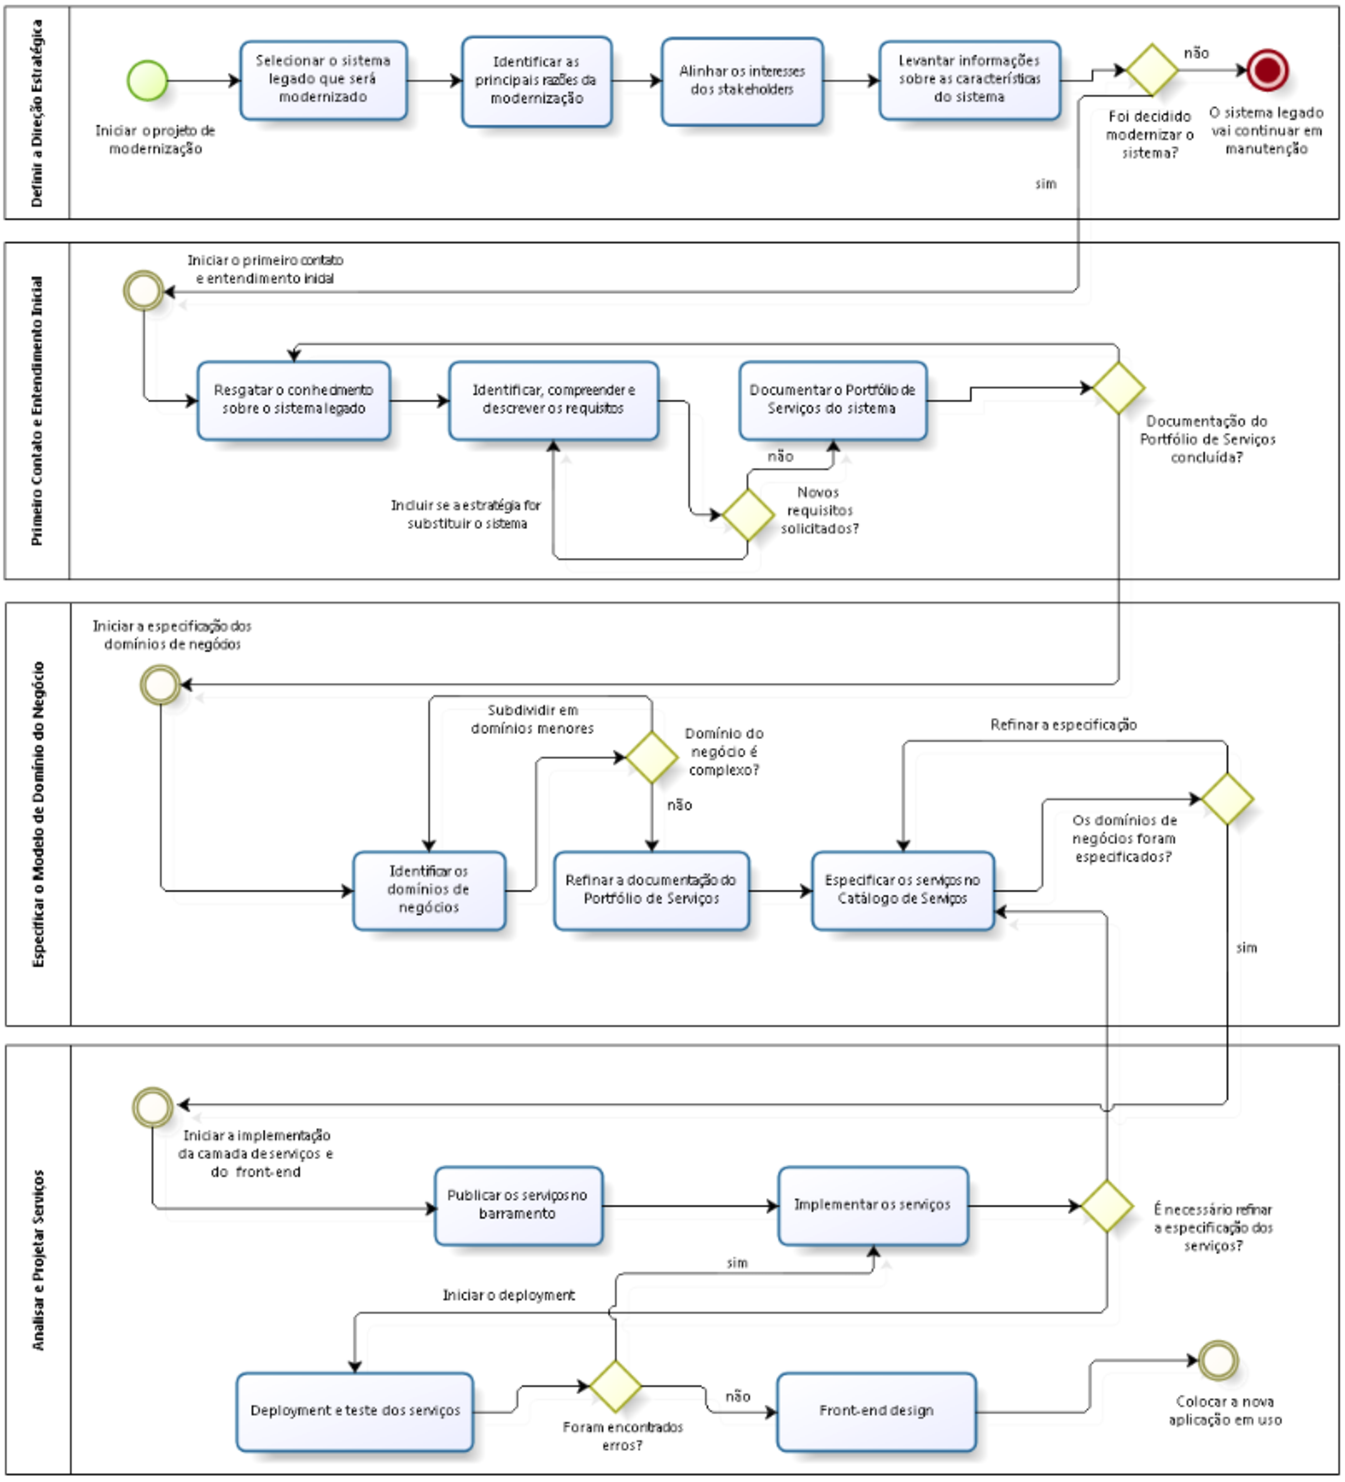
\includegraphics[scale=0.69]{img/processo/smsoc_processo.pdf}
\caption{SMSOC -- Processo de modernização de software proposto para o CPD/UnB.}
\label{fig:processo_erlangms}
\end{figure}

\FloatBarrier


Por outro lado, os fluxos de trabalhos \emph{Especificar o Modelo de Domínio do Negócio}
e \emph{Analisar e Projetar Serviços}
envolvem atividades mais técnicas como as de
especificação, implementação, testes e implantação (\textit{deployment}) 
da camada de serviços, além do desenvolvimento da interface visual da aplicação, 
referido como o \textit{front-end} no restante 
deste trabalho de dissertação. 


As atividades apresentadas a seguir e a 
arquitetura de software subjacente 
do processo,
fazem uso de algumas
práticas de design \acrshort{DDD} 
experimentadas durante o estudo de caso,
como por exemplo, o uso de uma linguagem 
ubíqua e o trabalho centrado em modelos de domínios de negócios
para auxiliar a equipe de modernização a raciocinar 
a camada de serviços da aplicação 
por meio de um conjunto de domínios de contexto
delimitados (ou \textit{Bounded Context})~\cite{evans2004domain}.

O restante desse capítulo tem a seguinte organização: 
As seções~\ref{pro:direcao},~\ref{pro:prim_contato},~\ref{pro:esp_modelo_dominio} 
e~\ref{pro:analisar_projetar}
descrevem os fluxos do processo,
incluindo a definição dos papéis envolvidos em cada etapa, 
os insumos ou artefatos de entrada, 
os artefatos produzidos e exemplos de condução de cada 
atividade com base no estudo de caso. 
Já, a seção~\ref{arquitetura}
apresenta a arquitetura do processo, 
descrevendo o design de implementação dos serviços
com exemplos de implementação (Subseção~\ref{design_implementacao}), 
os detalhes sobre o roteamento das 
mensagens (Subseção~\ref{roteamento}), as 
linguagens suportadas (Subseção~\ref{ling_suportada}), 
o modelo de computação adotado (Subseção~\ref{modelo_computacao}), 
a definição de um \textit{cluster} de serviços (Subseção~\ref{cluster_servico}), 
a especificação do catálogo de serviços (Subseção~\ref{catalogo_serviços}), 
alguns outros requisitos da arquitetura (Subseção~\ref{outros_req}) e 
um breve histórico sobre o desenvolvimento 
de um barramento de serviços para sustentar a abordagem proposta (Subseção~\ref{historico_barramento}).


\section{Definir a Direção Estratégica}\label{pro:direcao}


Como discutido em~\cite{S3_Bisbal:1999, 
Salvatierra:2013, WeidermanApproachesto:1997}, 
a modernização de um sistema legado é importante,
entre outros motivos,
para mantê-los alinhados 
com o negócio da organização, 
quando esses sistemas tornam-se
muito resistentes para manterem-se atualizados ou,
devido aos avanços tecnológicos ao longo dos anos.

Desse modo, havendo a necessidade de 
um projeto de modernização para o sistema legado,
é preciso antes de tudo,
estabelecer o direcionamento estratégico 
para identificar os objetivos e
a estratégia de modernização adequada.
Assim, a primeira atividade do processo
consiste em \emph{Definir a Direção Estratégica}, 
como está ilustrado na Figura~\ref{fig:direcao_estrategica}.

Durante a definição do direcionamento estratégico,
deve-se estabelecer o alinhamento de interesses 
entre os \textit{stakeholders} do projeto, 
que podem variar de organização 
para organização ou
talvez de projeto para projeto, uma vez que
muitos projetos são 
tipicamente onerados com interesses que puxam em diferentes direções, 
como negociais, econômicos, técnicos e também políticos,
como salienta~\cite{OORP2013}.

Para alcançar os objetivos 
do projeto de modernização, torna-se necessário
identificar as principais razões que levaram 
a organização a decidir por modernizar 
o sistema legado; alinhar os 
interesses dos \textit{stakeholders} para
definir os objetivos a curto e médio prazo e;
levantar algumas informações sobre as características 
do sistema legado. Todas essas informações
devem auxiliar a organização a refletir
sobre qual a melhor estratégia de modernização para o 
sistema legado. 

É importante destacar
que a ausência de um 
direcionamento estratégico pode levar 
a organização a optar por modernizar um sistema 
sem entender o motivo~\cite{S4_bennett1995legacy}. 
Por exemplo, alguns projetos realizados 
pelo CPD/UnB, como o \acrfull{SITRAN}, 
foram iniciados sem 
a presença dos \textit{stakeholders},
sendo bastante prejudicados, 
pois os objetivos do projeto não
estavam alinhados com as necessidades 
dos seus usuários que 
desconheciam que o sistema estava sendo modernizado.

Para auxiliar esta etapa, 
alguns questionamentos 
podem ser respondidos pelos \emph{especialistas do 
domínio de negócio} (\textit{stakeholders} e usuários)
em conjunto com os analistas e desenvolvedores do projeto.
Os questionamentos estão definidos na 
Tabela~\ref{tab:tabela_direcao_estrategica}
e de forma resumida, tem como objetivo
lançar alguns tópicos para a discussão
entre os envolvidos
com o intuito de obter as informações pertinentes 
do direcionamento estratégico, de modo que, 
o projeto possa ter continuidade. 

Sendo assim, como está destacado em negrito
na coluna \emph{Tópico de Análise}
na Tabela~\ref{tab:tabela_direcao_estrategica},
o questionário busca identificar
as expectativas com a
modernização do sistema legado, obter um 
entendimento em alto nível sobre o sistema e
conhecer os potenciais usuários desse sistema. 
Note que os tópicos de discussão poderão
ser ampliados conforme as necessidades do 
projeto de modernização.



% Tabela questionamentos para o direcionamento estratgico
%======================================================================================
\begin{table}[!htb]
\centering
\small
\caption{Questionamentos para auxiliar na direção estratégica.}
\label{tab:tabela_direcao_estrategica}
\begin{tabular}{|l|l|l|}
\hline
\rowcolor[HTML]{EFEFEF} 
\multicolumn{1}{|c|}{\cellcolor[HTML]{EFEFEF}\textbf{\begin{tabular}[c]{@{}c@{}}Tópico de \\ Análise\end{tabular}}}            & \multicolumn{1}{c|}{\cellcolor[HTML]{EFEFEF}\textbf{Questionamento Relacionado}}                                                                                                                                                             & \multicolumn{1}{c|}{\cellcolor[HTML]{EFEFEF}\textbf{Problema Potencial}}                                                                  \\ \hline
\cellcolor[HTML]{FFFFFF}\textbf{\begin{tabular}[c]{@{}l@{}}Expectativas com\\ a modernização\\ do sistema legado\end{tabular}} & \begin{tabular}[c]{@{}l@{}}Quais os principais fatores de\\ negócio que motivam a modernização?\\ \\ Quais os principais desafios\\ tecnológicos para alcançá-los?\\ \\ Quais os objetivos a curto\\ e médio prazo do projeto?\end{tabular} & \begin{tabular}[c]{@{}l@{}}Objetivos do projeto\\ não estão claros.\\ \\ Desafios tecnológicos\\ não foram identificados.\end{tabular}    \\ \hline
\textbf{\begin{tabular}[c]{@{}l@{}}Entendimento em\\ alto nível do\\ sistema legado\end{tabular}}                              & \begin{tabular}[c]{@{}l@{}}Qual é a principal funcionalidade\\ fornecida pelo sistema legado?\\ \\ Qual é a arquitetura em alto\\ nível do sistema legado?\\ \\ Quais interfaces com o\\ usuário são utilizadas?\end{tabular}                & \begin{tabular}[c]{@{}l@{}}Ausência de documentação\\ sobre o sistema legado.\\ \\ Arquitetura do sistema\\ não é conhecida.\end{tabular} \\ \hline
\textbf{\begin{tabular}[c]{@{}l@{}}Usuários potenciais \\ do sistema legado\end{tabular}}                                      & \begin{tabular}[c]{@{}l@{}}Quais são os usuários\\ do sistema legado?\end{tabular}                                                                                                                                                           & \begin{tabular}[c]{@{}l@{}}Não foram identificados\\ todos os usuários.\end{tabular}                                                      \\ \hline
\end{tabular}
\end{table}

Recomenda-se, com base na execução do estudo de caso,
que a execução desta atividade 
seja realizada com a maior brevidade possível, 
uma vez que a organização precisa definir o direcionamento
estratégico para que o projeto possa ter andamento.
Como observado em~\cite{S2_erlikh:2000},
se o sistema for considerado 
de grande porte ou muito complexo, 
a exemplo do
\acrfull{SIGRA} da \acrshort{UnB},
a modernização pode ser conduzida 
de maneira gradual, dividindo o 
projeto em partes ou em módulos.

No que se refere as possíveis entradas 
para a definição 
da direção estratégica, 
pode-se consultar, sempre que possível,
os manuais e as documentações sobre o sistema legado,
o próprio sistema legado, as capturas das telas e
as apresentações sobre o sistema,
entre 
outros artefatos ou insumos considerados úteis,
conforme ilustra a Figura~\ref{fig:direcao_estrategica}.
Salienta-se a importância dos \textit{stakeholders}, 
dos usuários, dos atuais mantenedores 
do sistema legado e da infraestrutura do 
ambiente de produção, 
bem como dos analistas e desenvolvedores nesse processo.
Note que, nem sempre vai haver
documentação atualizada sobre o sistema e 
os desenvolvedores
originais do sistema podem não estar mais na organização~\cite{S4_bennett1995legacy}.

Para obter um bom direcionamento estratégico
é crucial levantar algumas informações 
sobre a arquitetura do sistema (em alto nível) 
e identificar a principal funcionalidade do
sistema (para saber o que o sistema faz). 
Não havendo
pessoas que conhecem sobre a arquitetura do sistema 
e sobre os principais requisitos do negócio, 
essas informações podem
ser extraídas por meio de engenharia reversa, 
como sugere~\cite{OORP2013}. 


Esta atividade produz como saída
informações para auxiliar a organização a 
decidir a melhor estratégia de modernização, 
conforme mostra a Figura~\ref{fig:direcao_estrategica}. 
Assim,
com base nos levantamentos realizados, 
se torna possível identificar se a modernização será
uma migração, uma substituição ou se a organização 
vai continuar fazendo as manutenções evolutivas 
caso os custos ainda sejam justificáveis~\cite{S15_Comella-DordaASurvey2000}.
Além disso, executando esta atividade, 
é possível obter uma boa noção sobre o que
o sistema se propõe a resolver, identificar
a arquitetura do sistema legado em alto nível, 
as interfaces com o usuário disponíveis e quem são os
usuários desse sistema legado.

\begin{figure}[htb]
\centering
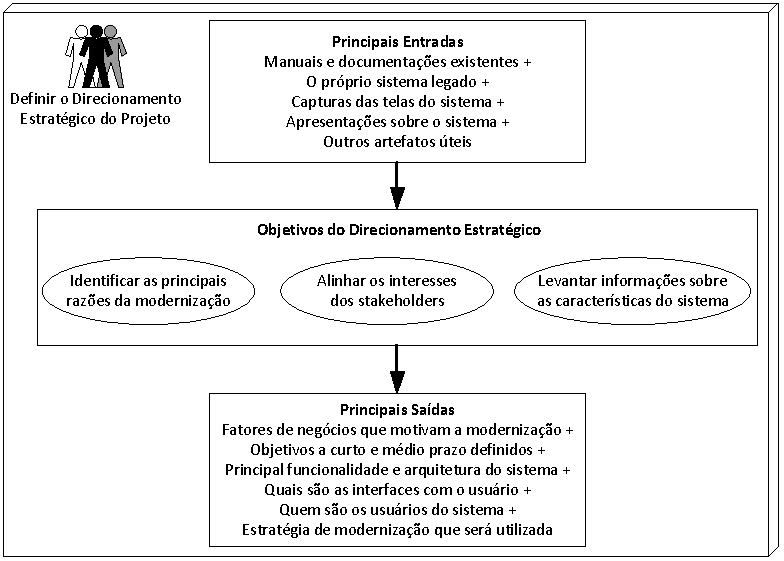
\includegraphics[scale=1]{img/processo/direcao_estrategica.pdf}
\caption{Definir a direção estratégica do projeto de modernização.}
\label{fig:direcao_estrategica}
\end{figure}


Para exemplificar, o 
direcionamento estratégico conduzido
durante o estudo de caso
é discutido a seguir.
Cabe esclarecer, que o questionário
proposto surgiu 
por meio de debates entre os participantes
do estudo de caso e gestores do CPD/UnB e, 
posteriormente, com os \textit{stakeholders}
e os usuários do \acrshort{SAE}.
Nesse estudo de caso, 
os tópicos de discussão propostos
mostraram-se suficientes para identificar 
a estratégia de modernização
a ser utilizada, que, neste projeto, consistiu em 
uma \emph{substituição} do sistema legado,
uma vez que se chegou a conclusão que o sistema 
deveria ser revisto para atender as demandas
dos usuários e por tratar-se de um sistema 
relativamente pequeno, seria possível reescrevê-lo 
durante o estudo de caso, caso contrário, seria realizado apenas a sua migração.

\begin{itemize}

\item Principais fatores de negócios que motivam a modernização.

Os principais
fatores considerados na modernização 
do \acrshort{SAE} envolvem
o alto custo de manutenção já que o sistema legado divide-se
em duas partes, sendo a primeira parte 
desenvolvida na linguagem VB e a segunda parte
em C\#. Além disso, existem funcionalidades que
estão duplicadas em ambas versões e 
quando há uma manutenção evolutiva, de acordo 
com o gerente da \acrshort{SSI}, 
geralmente, faz-se necessário modificar os dois códigos fontes. 
O \acrshort{SAE} é mantido por dois analistas do CPD/UnB, 
sendo que cada analista mantêm
uma versão do código fonte. Dessa forma, deseja-se unificar
os dois sistemas e ter apenas um único 
sistema para manter, facilitando a evolução
do sistema e o seu uso pelos usuários. Além disso,
o mantenedor da versão VB pode se aposentar nos próximos 3 anos.
Finalmente, os \textit{stakeholders} necessitam rever 
alguns requisitos de negócio para atender as demandas atuais.

\item Principais desafios tecnológicos para alcançá-los.

Além da dificuldade para criar os ambientes de desenvolvimento legados,
não foi encontrado nenhum outro 
desafio tecnológico nesse projeto uma vez que os mantenedores
do sistema legado ainda estão no CPD/UnB para 
auxiliar nos trabalhos de modernização.

\item Objetivos a curto e médio prazo do projeto.

Identificou-se três objetivos a curto prazo: 
a migração do sistema para a linguagem Java visando obter 
uma única base de código e 
facilitar a manutenção; a revisão dos requisitos do sistema junto 
aos usuários para satisfazer as necessidades atuais e finalmente,
testar a abordagem \acrshort{SOA} proposta neste trabalho de 
dissertação em um projeto de modernização real na Universidade.

Identificou-se um objetivo a médio prazo: a integração
do sistema \acrshort{SAE} 
com o \acrfull{SISRU}. Salienta-se que atualmente esta
integração se dá a nível de banco de dados e com esse projeto de modernização, 
será possível consumir um serviço em vez disso.

\item Principal funcionalidade fornecida pelo sistema legado.

A principal funcionalidade é o preenchimento da avaliação socioeconômica pelos estudantes 
da \acrshort{UnB} regularmente matriculados em disciplinas de cursos presenciais
de graduação e pós-graduação.


\item Arquitetura em alto nível do sistema legado.

A versão do sistema em VB possui uma arquitetura monolítica e as funcionalidades 
estão implementadas diretamente nos formulários (telas do sistema). 
A versão do sistema em C\# 
possui uma arquitetura monolítica também, mas o código fonte está organizado em três 
camadas. Além disso, a interface com o usuário está 
implementada em páginas web. Em ambas versões, 
existem regras de negócios
dentro do banco de dados através de \textit{stored procedures}.

\item Interfaces com o usuário utilizadas.

São utilizadas duas interfaces com o usuário. A versão VB do
sistema possui uma
interface desktop tradicional enquanto que a
versão C\# é um sistema web. O preenchimento da avaliação socioeconômica 
é realizada na versão C\#. A versão
VB do sistema é utilizada pelos administradores do \acrshort{PNAES} para 
fazer a gestão da avaliação bem como a emissão de relatórios diversos. 

\item Usuários do sistema legado \acrshort{SAE}.

Administradores do programa \acrshort{PNAES} e os estudantes da \acrshort{UnB}
regularmente matriculados em disciplinas de cursos presenciais
de graduação e pós-graduação. O sistema \acrshort{SISRU} também é um usuário
desse sistema, já que depende de informações geradas pelo sistema \acrshort{SAE}.

\end{itemize}


Com o direcionamento estratégico definido
e documentado, o processo pode seguir para a próxima etapa 
do processo, o \emph{Primeiro Contato e Entendimento Inicial}, 
no caso da organização ter optado pela modernização do sistema legado.




\section{Primeiro Contato e Entendimento Inicial}\label{pro:prim_contato}


O \emph{Primeiro Contato e Entendimento Inicial} 
representa o segundo fluxo de atividades
do processo \acrshort{SMSOC} e o
seu sucesso passa por resgatar o
conhecimento sobre o sistema legado 
que pode ter se perdido ao longo dos anos com a 
evolução natural do software decorrente 
das manutenções evolutivas sem a devida documentação.
A Figura~\ref{fig:primeiro_contato} mostra o 
esquema dessa atividade com as entradas, 
os objetivos e saídas definidos.


Considerando a literatura
~\cite{S4_bennett1995legacy, S3_Bisbal:1999, Chikofsky:1990, Comella:2000, OORP2013},
esta atividade pode ser desempenhada 
por meio de entrevistas com os especialistas no
domínio do negócio da aplicação 
(os \textit{stakeholders}, usuários e 
mantenedores do sistema legado);
aplicando engenharia reversa
no código-fonte ou no esquema do bancos de 
dados do sistema legado (que pode ser feito manualmente ou com o apoio
de ferramentas de análise estática);
analisando o comportamento do sistema legado observando
suas interfaces externas, entre outras formas.


Para a execução desta atividade, 
não foi definido um prazo máximo 
para ser concluída,
uma vez que isso pode depender de vários fatores verificados na literatura, 
como salientam~\cite{S4_bennett1995legacy, S3_Bisbal:1999, S04_IntLgSw:2006}, 
tais como 
o tamanho e a complexidade do software legado,
a existência de documentação atualizada 
ou de especialistas no domínio do negócio. 
No caso do CPD/UnB, 
além dos fatores mencionados,
existe certa dificuldade em reunir 
os \textit{stakeholders} por conta da disponibilidade de cada um.


De acordo com~\cite{S4_bennett1995legacy, S3_Bisbal:1999}, 
será necessário obter uma boa 
compreensão do sistema legado para
gerar a documentação sobre este sistema. 
Os autores~\cite{S4_bennett1995legacy, clements2002documenting} evidenciam
que um dos maiores desafios dessa atividade pode ser 
localizar os conceitos
de domínio do negócio no sistema legado.
Nesse caso, como é possível presumir,
a participação dos especialistas do 
domínio do negócio será muito importante.
Entretanto, é possível que alguns especialistas do negócio
não façam mais parte da organização, 
o que deve dificultar a condução desta atividade~\cite{S4_bennett1995legacy}.


\begin{figure}[htb]
\centering
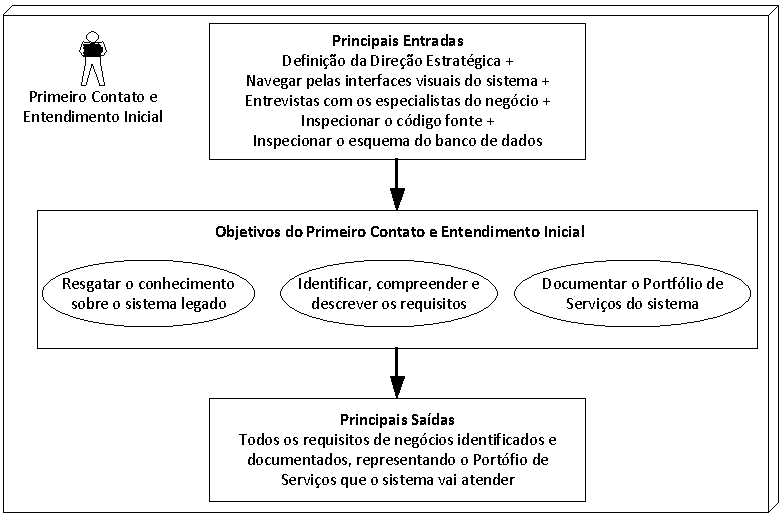
\includegraphics[scale=1]{img/processo/primeiro_contato.pdf}
\caption{Primeiro contato e entendimento inicial do projeto de modernização.}
\label{fig:primeiro_contato}
\end{figure}


É oportuno ressaltar,
um inconveniente 
que se observa na \acrshort{UnB} e 
possivelmente em outras Instituições: 
parte do conhecimento
sobre os sistemas legados
estão na forma tácita adquiridos ao 
longo das experiências e vivências 
das pessoas que se envolveram com esses sistemas 
e que ainda trabalham na organização.
Em vista disso, percebe-se que esta atividade não só 
será o principal insumo de entrada para a próxima etapa
do processo, a \emph{especificação do domínio de negócio},
como proverá o resgate 
do conhecimento tácito
para uma forma explícita.

Como pode-se ver na Figura~\ref{fig:primeiro_contato},
o processo \acrshort{SMSOC} 
seleciona algumas técnicas identificadas na literatura
para serem utilizadas no 
primeiro contato e o entendimento inicial como 
entradas para esta atividade. Salienta-se que 
essas técnicas foram validadas 
e mostraram-se mais eficazes 
quando aplicadas
em conjunto, embora outras técnicas possam 
ser utilizadas conforme a necessidade do projeto.

\begin{itemize}

	\item Navegar pelas interfaces visuais do sistema legado. 

A navegação pelas interfaces do sistema 
legado foi a primeira técnica utilizada,
uma vez que os participantes do estudo de caso 
não tinham nenhum conhecimento 
sobre o sistema legado e também 
não havia documentação atualizada. 
Como observado em~\cite{S12_WeidermanApproaches:1997},
esta técnica compreende uma abordagem
\textit{Black-box}, através do qual, a compreensão do sistema 
envolve analisar as interfaces externas do sistema legado
com base nas entradas fornecidas e saídas produzidas.

	\item Entrevistas com os especialistas do domínio de negócio.

As entrevistas com os especialistas do negócio 
são de suma importância
para a compreensão dos requisitos da aplicação~\cite{OORP2013}. 
A abordagem \acrshort{DDD} sugere 
o uso de uma linguagem ubíqua na
comunicação dos desenvolvedores
com os especialistas do negócio para
que os termos utilizados no domínio 
do sistema sejam compreendidos por todos,
tanto na comunicação falada, 
na documentação e no próprio código fonte
do sistema~\cite{evans2004domain}.
Como se identificou no estudo de caso, nem sempre vai 
ser possível entender plenamente o funcionamento de 
um sistema legado
sem a presença dos especialistas. 
Assim sendo, recomenda-se que sejam convocadas
algumas reuniões com os especialistas para que eles apresentem
passo a passo o funcionamento do sistema legado, 
dando a oportunidade para que os analistas 
levantem os requisitos e tirem as dúvidas que surgirem.


	\item Inspecionar o código fonte do sistema legado.
	
É bastante comum os responsáveis pelo
desenvolvimento e manutenção dos sistemas legados
dependerem do código fonte para compreendê-los
e posteriormente, efetuar as manutenções
evolutivas solicitadas pelos usuários, 
principalmente quando não há documentação ou 
a documentação está desatualizada~\cite{S01_bennett2000software,S3_Bisbal:1999, Seacord:2003, S04_IntLgSw:2006}.
Assim, nesses sistemas,
cujo código fonte ainda é o único
meio para obter o conhecimento sobre
as regras de negócios, 
como é o caso 
de muitos dos sistemas legados
desenvolvidos pelo CPD/UnB ao longo de 20 anos,
o uso do mesmo para compreender 
o seu funcionamento deverá prevalecer até que exista
uma documentação que reflita efetivamente
os requisitos de negócios desses sistemas.

No estudo de caso, os participantes inspecionaram o
código fonte do \acrshort{SAE} (tanto a versão VB quanto a versão C\#) 
com o auxílio de ferramentas de análise estática,
o que ajudou a identificar os principais
artefatos no código fonte e levantar algumas 
métricas sobre o sistema, tais como o número de linhas de código (LoC) e 
a complexidade ciclomática que 
mede a complexidade de um software contando 
o número de caminhos diferentes que um método 
pode ter~\cite{mccabe1976complexity}.
Pode-se dizer que a inspeção do código fonte 
foi interessante mas, 
na visão dos participantes do estudo de caso,
a inspeção do esquema do banco de dados revelou-se mais útil, 
conforme identificado na avaliação realizada no Capítulo~\ref{avaliacao}.
Contudo, torna-se necessário enfatizar que 
surgiram dúvidas em alguns requisitos que nem
mesmo os especialistas souberam responder, sendo
necessário recorrer
ao código fonte do sistema legado, mostrando que mesmo mais complexo 
para extrair as regras de negócio, as vezes, é a única alternativa.


	\item Inspecionar o esquema do banco de dados do sistema legado.
	
A inspeção do esquema do banco de dados 
foi uma das técnicas 
mais utilizadas na modernização do \acrshort{SAE} e
em conjunto com as técnicas anteriores,
possibilitou compreender melhor os requisitos de negócios. 
Na avaliação conduzida
no Capítulo~\ref{avaliacao}, constatou-se que isso se deve
ao fato de que, após obter uma boa compreensão do que o sistema faz 
com a ajuda dos especialistas do negócio, 
ficou mais fácil entender os detalhes do sistema 
analisando as tabelas e seus relacionamentos, 
até mesmo para auxiliar na especificação do domínio do 
negócio, como será discutido na próxima atividade do processo. 
Nesse sentido, com base na experiência obtida
durante o estudo de caso,
recomenda-se que a equipe do projeto de modernização
analise em conjunto
as estruturas do esquema
do banco de dados da aplicação, 
pois pode-se mostrar uma fonte
valiosa para conhecer o sistema legado.

	

\end{itemize}


 
Esta atividade gera uma documentação 
abrangente descrevendo as 
funcionalidades do sistema legado e os 
requisitos de negócios identificados, 
denominado de \emph{Portfólio de Serviços} 
do projeto de modernização.
De acordo com a Figura~\ref{fig:portfolio_servicos},
o Portfólio dos Serviços 
lista as funcionalidades
que serão implementadas no 
sistema descritas 
de forma concisa e clara. No estudo 
de caso utilizou-se um quadro \emph{Kanban}
usando a ferramenta 
\emph{Trello}, disponível 
no sítio  \url{https://trello.com}, 
possibilitando aos participantes
criar o Portfólio de Serviços
e gerenciá-lo através de cartões (\textit{boards}), os quais
foram úteis também para 
documentar as atividades do projeto,
adicionar comentários, links, imagens e 
salvar anexos dos modelos criados, 
além de permitir determinar os prazos para execução 
das atividades do projeto de modernização do \acrshort{SAE}.


\begin{figure}[htb]
\centering
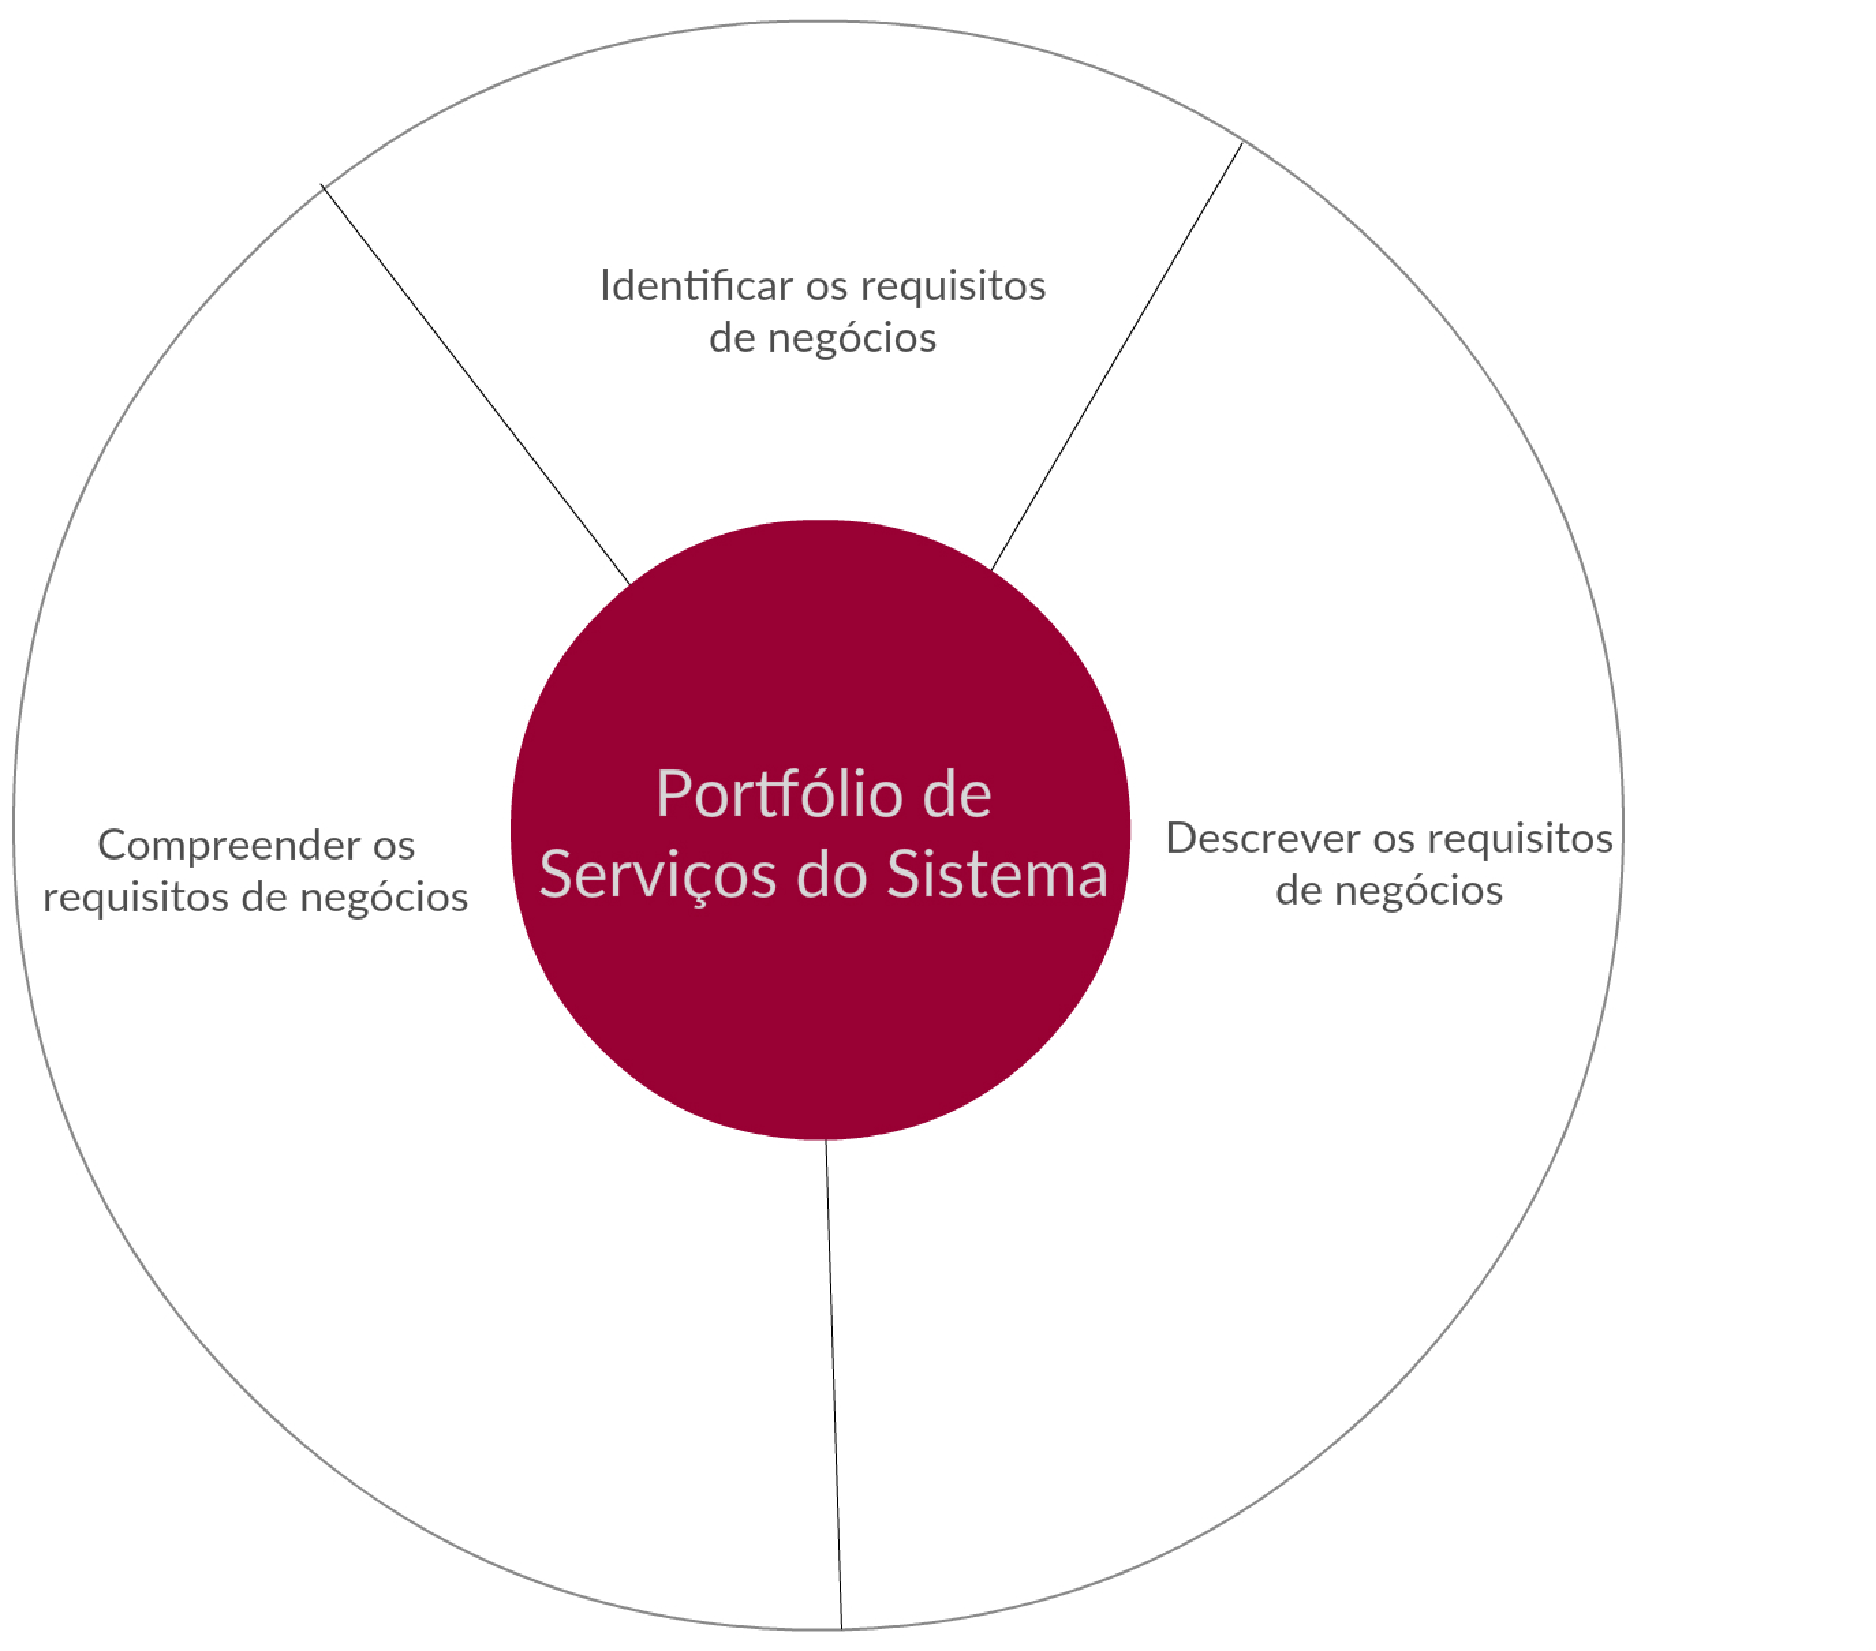
\includegraphics[scale=0.30]{img/processo/portfolio_servicos.pdf}
\caption{Portfólio de Serviços do projeto de modernização.}
\label{fig:portfolio_servicos}
\end{figure}


Antes de passar para a próxima atividade do processo, 
salienta-se que novas
funcionalidades ou mudanças nos requisitos de negócios 
podem ser solicitados,
como ocorreu com o \acrshort{SAE}. 
Assim, 
dependendo da estratégia de modernização
adotada pela equipe, que pode ser uma migração, 
uma substituição ou 
continuar mantendo 
o sistema legado~\cite{S3_Bisbal:1999, Seacord:2003, S12_WeidermanApproaches:1997}, 
a nova funcionalidade ou o requisito
poderá ou não ser implementado
durante o projeto de modernização.
Nesse caso, os autores~\cite{S3_Bisbal:1999, Seacord:2003}
recomendam que se a opção escolhida for pela a migração do sistema, 
deve-se inicialmente preservar as funcionalidades e 
os dados (caso contrário, representará uma substituição)
e implementar as novas demandas após 
o sistema entrar em produção para facilitar os testes da aplicação.










\section{Especificar o Modelo de Domínio do Negócio}\label{pro:esp_modelo_dominio}

A partir desta etapa do projeto, 
pode-se
iniciar a especificação 
da camada de serviços do software
com a documentação gerada
no Portfólio de Serviços, 
conforme mostra a Figura~\ref{fig:dominio_negocio}.
Pode-se dizer que o principal produto 
gerado da especificação,
são os modelos de domínio do negócio, 
os quais
representam uma abstração do problema
que será solucionado pelo 
sistema e o ponto central onde concentram-se
grande parte da complexidade inerente ao 
software, na visão de~\cite{S3_Bisbal:1999, S01_bennett2000software, evans2004domain, fowler2002patterns}. 

Como foi visto no \acrshort{MS},
muitas vezes as organizações 
focam-se muito mais nos aspectos técnicos,
arquiteturais e tecnológicos do software 
do que em compreender
e modelar os domínios da aplicação
de forma aprofundada. 
Sendo a especificação 
dos domínios de negócio
uma das partes
mais complexas
na modernização do software~\cite{evans2004domain},
propõem-se
organizar a lógica do negócio
como o uso dos padrões
de design
\textit{Domain Model},
que consiste na
modelagem de
modelos ricos (ou seja, o sistema
é composto por um conjunto de objetos 
que possui comportamentos e são inter-relacionados);
e o \textit{Bounded Context},
que consiste 
em delimitar (baseados nas intenções do negócio) um domínio grande
em domínios menores
para diminuir a complexidade da solução~\cite{fowler2002patterns}.


Para suportar esta organização,
o processo \acrshort{SMSOC} sugere
que os modelos de domínio do negócio
desenvolvidos estejam
contidos dentro de módulos
(ou pacotes) de software, 
representando os \textit{Bounded Context}.
Entretanto, cabe esclarecer,
segundo~\cite{avram2007domain},
que um \textit{Bounded Context} 
não é um módulo de software, 
já que seu objetivo é
fornecer um recipiente lógico para os modelos,
enquanto os módulos de software são utilizados 
para organizar os elementos (ou artefatos)
de um software,
sendo, 
de acordo com~\cite{clements2002documenting}, 
uma unidade
de implementação para o software, 
que disponibiliza
uma unidade coerente de funcionalidades.
Para simplificar, no restante
deste capítulo será utilizado o 
termo módulo referindo-se
igualmente a um \textit{Bounded Context}, uma vez que,
na arquitetura proposta, um \textit{Bounded Context}
é manifestado dessa forma.


\begin{figure}[htb]
\centering
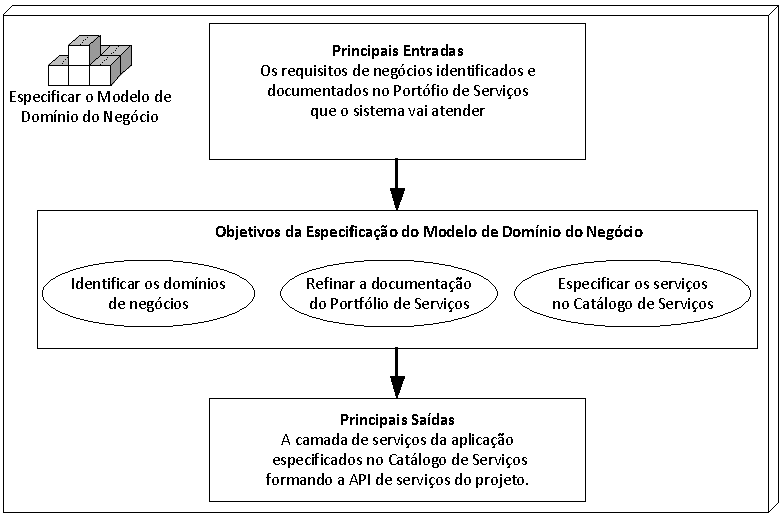
\includegraphics[scale=1]{img/processo/dominio_negocio.pdf}
\caption{Especificar o modelo de domínio do negócio.}
\label{fig:dominio_negocio}
\end{figure}

Faz-se necessário enfatizar
que em termos de código fonte, 
a manifestação dos modelos 
de domínio do negócio tem lugar
na camada de serviços (camada que contém a lógica negocial)
dos módulos desenvolvidos com a abordagem proposta.
Mais detalhes serão 
apresentados
na atividade \emph{Analisar e Projetar Serviços},
mas, apenas para adiantar, 
os módulos neste trabalho podem ser vistos
como uma estrutura 
de objetos 
organizados em três camadas (Fachada, Serviço e Infraestrutura),
que refletem o modelo de domínio do negócio
especificado
para tirar proveito
dos benefícios da orientação a objetos.



Um conceito fundamental do \acrshort{DDD}
é subdividir
um grande modelo de negócio
em domínios menores~\cite{evans2004domain}. 
Para exemplificar, 
a modernização
do \acrshort{SAE} resultou em 4 
módulos representando
os \textit{bounded context}, 
como mostra a Figura~\ref{fig:bound_context}: o \emph{unb-questionario}   
surgiu devido a possibilidade de se criar um conjunto de serviços para
gestão de questionários genéricos, permitindo o seu uso em outros sistemas
além do \acrshort{SAE} (requisito solicitado pelo CPD); o módulo
\emph{unb-sae} contém os serviços para a
avaliação socioeconômica dos estudantes do programa \acrshort{PNAES} e os
módulos \emph{unb-sigra} e \emph{unb-sitab} contém
alguns serviços necessários para o sistema.

\begin{figure}[htb]
\centering
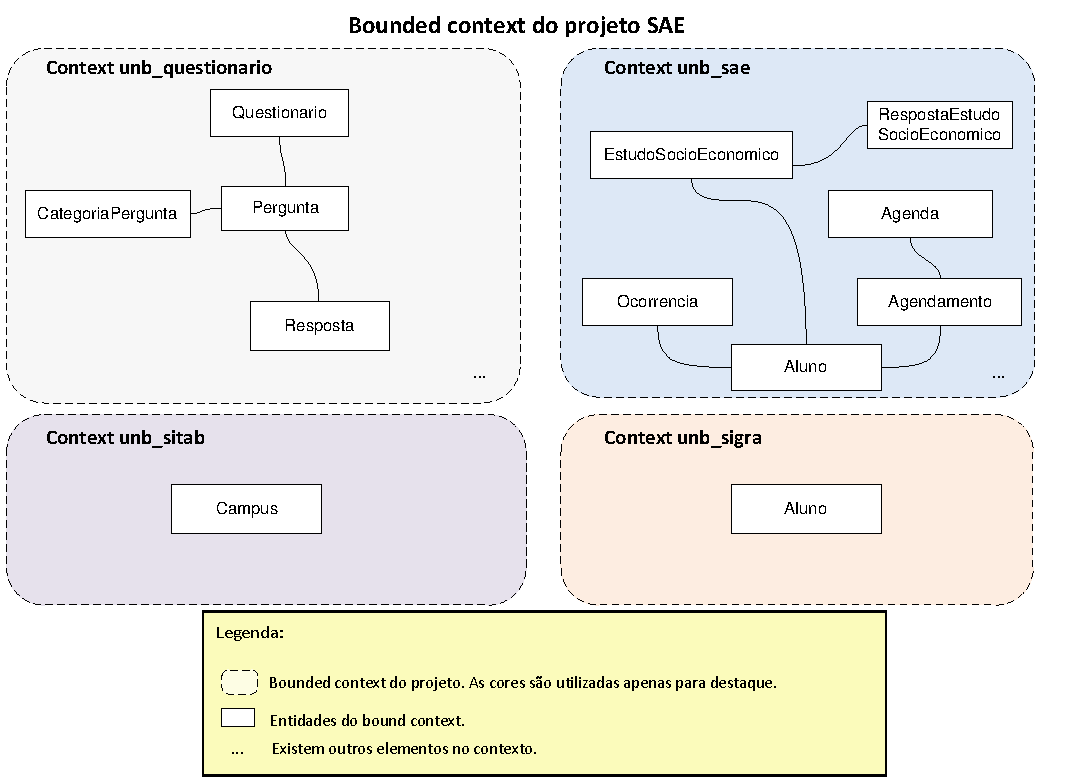
\includegraphics[scale=0.91]{img/processo/bound_context.pdf}
\caption{Módulos do projeto SAE representando os bounded context.}
\label{fig:bound_context}
\end{figure}

Outro conceito do \acrshort{DDD} utilizado
no estudo de caso foi
o uso da linguagem ubíqua para
expressar os termos 
do domínio como os especialistas se referem,
possibilitando 
criar um vocabulário comum que todos do projeto entendem~\cite{evans2004domain}. 
A Figura~\ref{fig:exemplo_entidade}
ilustra esse aspecto, 
onde os métodos declarados na classe \emph{Aluno}
implementada para o \acrshort{SAE}
refletem o comportamento desejado
de acordo com os termos utilizados 
pelos especialistas do negócio. 
Além disso, pode-se reparar 
também que a classe representa
um objeto rico (ou um objeto que não é anêmico),
conceito fundamental para 
a modelagem de domínios no processo \acrshort{SMSOC}. 

Na visão de~\cite{balasubramanian2006developing},
objetos anêmicos são aqueles que possuem somente atributos
e os métodos ficam espalhados no sistema
formando um modelo anêmico e procedural e
que segundo~\cite{evans2004domain},
pode ser um sinal de que a equipe 
não está fazendo uso de \acrshort{DDD} ou 
possa ser uma falha no
processo de modelagem. 


\begin{figure}[htb]
\centering
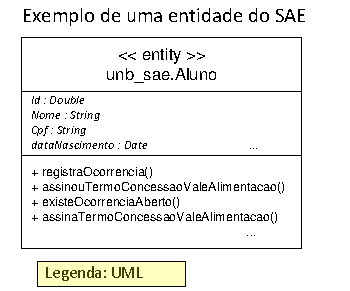
\includegraphics[scale=1.4]{img/processo/exemplo_classse_aluno.pdf}
\caption{Exemplo de uma entidade não anêmica do \acrshort{SAE}.}
\label{fig:exemplo_entidade}
\end{figure}





Lista-se a seguir, algumas diretrizes
para execução 
desta atividade que foram definidas
com base nas experiências 
adquiridas pelos participantes do estudo de caso,
com o uso de algumas práticas \acrshort{DDD}
descrito na 
literatura~\cite{balasubramanian2006developing, evans2004domain, fowler2002patterns, vernon2013implementing}. 

\begin{itemize}

\item Interagir com os especialistas do domínio

A primeira diretriz consiste em interagir com 
os especialistas do domínio logo ao 
iniciar um projeto de modernização. 
O trabalho com os especialistas 
possibilitará resgatar o conhecimento sobre o 
sistema legado e documentá-los no 
Portfólio de Serviços, para então, 
especificar o domínio do negócio. 
Segundo~\cite{fowler2002patterns},
recomenda-se que um domínio complexo seja 
quebrado em subdomínios menores
com a ajuda dos especialistas, os quais
serão os módulos da camada de serviços da aplicação.

\item Especificar os domínios centrado em serviços

No processo \acrshort{SMSOC},
os domínios do negócio 
são orientados a serviços de 
acordo com a abordagem proposta. Esta
é uma recomendação adotada
para o processo pois
segundo enfatizado
em~\cite{evans2004domain},
alguns projetistas centram-se na modelagem 
dos dados ao invés da lógica do negócio. 
Note que,
essa recomendação não foi inicialmente seguida
no estudo de caso pois 
os participantes
estavam modelando os domínios do negócio
a partir de uma
abordagem \textit{Transaction Script}.
Novamente, convém salientar que
houve uma paralisia da análise no início
da especificação dos domínios
do negócio do \acrshort{SAE},
pois os membros do projeto ainda
não tinham decidido utilizar a abordagem
\acrshort{DDD} uma vez que
os sistemas desenvolvidos pelo CPD/UnB
até então utilizavam o 
design \textit{Transaction Script},
já bem conhecido pelos 
desenvolvedores da \acrfull{SSI} do \acrshort{CPD}. 
Mais informações sobre 
\textit{Transaction Script} podem
ser obtidos no Capítulo~\ref{fundamentos} 
deste trabalho.



\item Usar a linguagem dos especialistas do domínio

Essa recomendação já foi enfatizada 
anteriormente neste capítulo e
consiste em usar uma linguagem compartilhada 
com os especialistas do domínio do negócio (linguagem ubíqua).
Nesse caso,
essa linguagem precisa ser aplicada
tanto na comunicação com os especialistas, 
no portfólio de serviços, 
quanto no código fonte do sistema, 
por meio de nomes de classes e métodos.

\item Identificar a fronteira e a limitação dos contextos

De acordo com~\cite{evans2004domain},
pode-se resolver os problemas complexos 
dividindo-os
em partes menores, 
para que seja possível
trabalhar uma parte mais coesa e com menor complexidade de cada vez.
Os participantes do estudo de caso seguiram 
esta diretriz e criaram 4 domínios de contexto
delimitado, cada um representando um módulo
da camada de serviços do \acrshort{SAE}. 
O principal resultado percebido disso
foi simplificar o desenvolvimento dos serviços.



\end{itemize}

Seguindo as diretrizes apresentadas,
como pode-se ver na Figura~\ref{fig:dominio_negocio},
será possível especificar 
os modelos de domínio do negócio
na forma de uma \acrfull{API} para os serviços
que serão posteriormente implementados
em alguma linguagem de programação. 
Note que a especificação dos 
serviços desses modelos possui uma atividade
de construção específica para isso,
denominado \emph{Especificar o Catálogo de Serviços},
que será discutida logo a seguir.




\section{Analisar e Projetar Serviços}\label{pro:analisar_projetar}

\emph{Analisar e Projetar Serviços}
consiste nas atividades de construção 
do projeto
que vai resultar no desenvolvimento 
de um conjunto de serviços 
representando a camada de serviços
da aplicação (ou \textit{back-end}) 
e no desenvolvimento do \textit{front-end} 
para permitir a interação dos usuários 
com os serviços oferecidos.

A Figura~\ref{fig:processo_erlangms}
mostra várias atividades de construção
no processo, iniciando pela
especificação dos catálogos de serviços
até a implementação e \textit{deployment}
dos serviços. 
Outras atividades podem
ser executadas além das definidas 
neste processo.
Note também que
esta atividade pode envolver tarefas
de análise também conforme a 
necessidade do projeto, talvez para um 
refinamento das especificações dos domínios.

É importante salientar que
o projeto dos serviços 
pode ser iniciado tão logo a
equipe tenha 
o Portfólio de Serviços. 
Por exemplo, os participantes 
do estudo de caso 
iniciaram de forma preliminar 
a construção dos serviços
durante a especificação do domínio 
do negócio, permitindo
verificar se a modelagem das APIs 
atendia aos requisitos 
do negócio de forma adequada.
Tal abordagem possibilitou também esclarecer 
dúvidas na forma de 
especificar um determinado serviço.

Para exemplificar esse aspecto no estudo de caso,
na especificação dos serviços
\emph{agenda} e \emph{agendamento} 
para uma entrevista (dois serviços 
essenciais do \acrshort{SAE} para cadastrar uma 
agenda com os dias/horários disponíveis 
para atendimento e;
permitir que o estudante solicite
um atendimento em determinado dia/hora),
haviam dúvidas
sobre a especificação mais 
adequada desses serviços. 
Ou seja,
qual seria a URL e os parâmetros de entrada do serviço,
tais parâmetros seriam passados na \textit{querystring} 
ou no \textit{payload} da requisição ao serviço. Ainda,
ao cadastrar uma agenda com todos os dias/horários possíveis
seriam necessários apenas uma invocação ao serviço \emph{agenda}
ou então vários-- uma requisição para cada dia/hora a ser cadastrado. 

Para resolver essas e outras dúvidas,
os participantes lançaram mão de várias ideias para auxiliar
na solução,
como imaginar a interação do usuário com 
as telas do sistema ou
imaginar os serviços com base no modelo
relacional (identificando quais tabelas seriam necessárias).
Por fim, a solução somente foi posta a prova
quando os contratos dos serviços foram especificados nos catálogos de serviços. 
Essa estratégia possibilitou a equipe 
testar\footnote{Utilizou-se a ferramenta REST Advanced REST Client para os testes.} e
visualizar o comportamento dos serviços, 
auxiliando tanto
no design final dos serviços como também em sua compreensão.
Note que, para testar os serviços especificados,
a equipe prototipava uma implementação preliminar do serviço, que geralmente 
consistia apenas na fachada dos serviços.

Por fim, sendo esta atividade de projeto essencialmente de construção,
apresenta-se a seguir, as principais atividades que foram definidas 
no processo \acrshort{SMSOC}, salientando novamente que podem existir outras atividades 
não listadas neste trabalho.


\subsection{Especificar o Catálogo de Serviços}

O objetivo desta atividade 
é prover a \acrshort{API} de serviços da aplicação por meio
da definição dos contratos de serviços 
no catálogo de serviços. Para isso,
deve-se especificar os serviços
através de metadados,
como a URL,
o tipo de serviço 
REST (\textit{GET, POST, PUT, DELETE}), 
os parâmetros do serviço, 
o dono do serviço (ou responsável), 
entre outras informações. 

O catálogo de serviços contém as definições para 
os serviços 
que serão disponibilizados aos usuários 
e tem como objetivo permitir 
a separação da especificação dos serviços
da sua implementação. Esses catálogos
são, essencialmente arquivos texto 
no formato JSON que seguem um 
determinado layout definido na Seção~\ref{arquitetura}.

Para ilustrar o trabalho no \acrshort{SAE}, 
o Código~\ref{fig:catalogo_processo} 
exibe parte da definição de um serviço 
denominado \emph{servico\_preliminar} 
do domínio do negócio \emph{unb\_sae}. 
Note como os metadados são utilizados para especificar 
os serviços listados.
As definições completas 
estão no sítio \url{https://github.com/erlangMS/msbus/tree/master/priv/conf/catalog}.

Segundo~\cite{RestApiDesign:2011},
projetar uma \acrshort{API}
não é somente pensar em aspectos 
de implementação, 
o design do serviço
é importante e
enquanto alguns metadados 
definidos para o design dos 
serviços
são essencialmente características 
de implementação do serviço, 
como o atributo \textit{lang}, 
que indica a linguagem 
de implementação do serviço
ou talvez \textit{async}, que indica
que o serviço é assíncrono,
outros atributos
como a \textit{url} e o \textit{type}, 
expressam o design do serviço, 
ou seja, como o cliente do serviço vai acessá-lo.

Como foi visto na literatura~\cite{flanders2008restful},
recomenda-se a adoção
de um design consistente e uniforme 
para o design dos serviços, 
caso contrário,
existe a possibilidade de 
cada projetista fazê-lo de uma forma. 
Para garantir um design uniforme, a equipe
deve revisar em conjunto 
as especificações dos serviços
como ocorreu no \acrshort{SAE}.

Em virtude do que foi mencionado,
apenas para exemplificar o design e
principalmente, o formato 
das URLs dos serviços do \acrshort{SAE},
pode-se ver no
Código~\ref{fig:catalogo_processo} 
que foi adotado um esquema orientado a objetos.
Note que para lançar uma 
resposta para um determinado 
estudo preliminar, primeiramente 
deve-se informar no parâmetro \emph{:id} 
o estudo preliminar, 
sendo que, se existir um estudo preliminar
com id igual a 100, por exemplo,
uma requisição para a \acrshort{URL}
\emph{/sae/estudo\_preliminar/100/resposta} 
vai permitir lançar uma resposta para o estudo preliminar correspondente.



\lstset{
        basicstyle=\footnotesize,
        numbers=left,
        numberstyle=\footnotesize,
        tabsize=2,
        numbers=none,
        rulesepcolor=\color{blue}}
\renewcommand{\lstlistingname}{Código}             
\begin{lstlisting}[caption=Especificação parcial da API do serviço estudo\_preliminar., label=fig:catalogo_processo] 
{
  "name": "/sae/estudo/preliminar/:id/resposta",
	"comment": "Cadastrar resposta do estudo preliminar",
	"owner": "sae",
	"service" : "br.unb.sae.facade.EstudoPreliminarFacade:insertResposta",
	"url": "/sae/estudo/preliminar/:id/resposta",
	"type": "POST"
},

{
  "name": "/sae/estudo/preliminar",
	"comment": "Pesquisar estudo preliminar",
	"owner": "sae",
	"service" : "br.unb.sae.facade.EstudoPreliminarFacade:find",
	"url": "/sae/estudo/preliminar",
	"type": "GET",
	"async":"false",
	"lang" : "java"
	"querystring": [
		{
			"name": "filtro",
			"type": "string",
			"default" : "",
			"comment": "Filtro principal da pesquisa"
		},
		{
			"name": "fields",
			"type": "string",
			"default" : "",
			"comment": "Campos que devem ser retornados na pesquisa"
		},
		{
			"name": "limit_ini",
			"type": "int",
			"default" : "0",
			"comment": "Limite inicial do paginador"
		},
		{
			"name": "limit_fim",
			"type": "int",
			"default" : "100",
			"comment": "Limite final do paginador"
		},
		{
			"name": "sort",
			"type": "string",
			"default" : "",
			"comment": "Campos que devem ser ordenados"
		}
	]
},

\end{lstlisting}


\subsection{Publicar os Serviços no Barramento}

A publicação dos serviços 
no barramento deve ser realizada para que  
estejam disponíveis aos usuários, entre eles, o próprio
\textit{front-end} da aplicação.
A publicação do serviço, antes 
de sua implementação permite
informar ao barramento 
onde estão localizados fisicamente no
sistema de arquivos do servidor, 
os catálogos de serviços 
que foram especificados, 
de modo que o 
módulo \textit{Dispatcher}
do barramento possa 
rotear as requisições \acrshort{REST} 
para os serviços solicitados pelos usuários.

A arquitetura proposta neste trabalho
suporta vários 
catálogos de serviços
dependendo da necessidade 
do projetista.
Por exemplo, inicialmente
os analistas do \acrshort{SAE} 
tinham definido
um único catálogo de serviços
que tornou-se rapidamente 
complexo de gerenciar e
suscetível a erros, sendo que
a equipe acabou decidindo dividir
em catálogos menores, um para cada serviço identificado.

Para informar a localização dos 
catálogos de serviços
é preciso editar o
\emph{catálogo mestre} do barramento. 
Um exemplo desse arquivo 
pode ser visualizado no 
Código~\ref{fig:catalogo_mestre},
através do qual, pode-se verificar que 
existem várias entradas 
informando ao barramento onde encontra-se
cada catálogo de serviço definido para o sistema.


\lstset{
        basicstyle=\footnotesize,
        numbers=left,
        numberstyle=\footnotesize,
        tabsize=2,
        numbers=none,
        rulesepcolor=\color{blue}}
\renewcommand{\lstlistingname}{Código}             
\begin{lstlisting}[caption=Exemplo do catálogo mestre do projeto SAE., label=fig:catalogo_mestre] 
[
	{
		"catalog": "/sae/catalogo_estudo_preliminar", 
		"file": "sae/catalogo_estudo_preliminar.conf"
	},
	
	{
		"catalog": "/sae/catalogo_estudo_socioeconomico", 
		"file": "sae/catalogo_estudo_socioeconomico.conf"
	},
	
	{
		"catalog": "/questionario/categoria", 
		"file": "questionario/catalogo_categoria_pergunta.conf"
	},

	{
		"catalog": "/questionario/pergunta", 
		"file": "questionario/catalogo_pergunta.conf"
	}
]
\end{lstlisting}


Foi implementada uma versão inicial de um \emph{Portal de Serviços Web} 
com a finalidade de
permitir a consulta dos catálogos de 
serviços especificados, 
tanto pelos desenvolvedores quanto pelos 
potenciais usuários.
Funcionalidades adicionais serão 
introduzidas a este portal, para permitir, 
por exemplo,
a especificação dos catálogos sem precisar editar 
os arquivos diretamente. 
A Figura~\ref{fig:portal_servicos}
exibe a interface visual desse portal
com a lista de alguns serviços do \acrshort{SAE}.

\begin{figure}[htb]
\centering
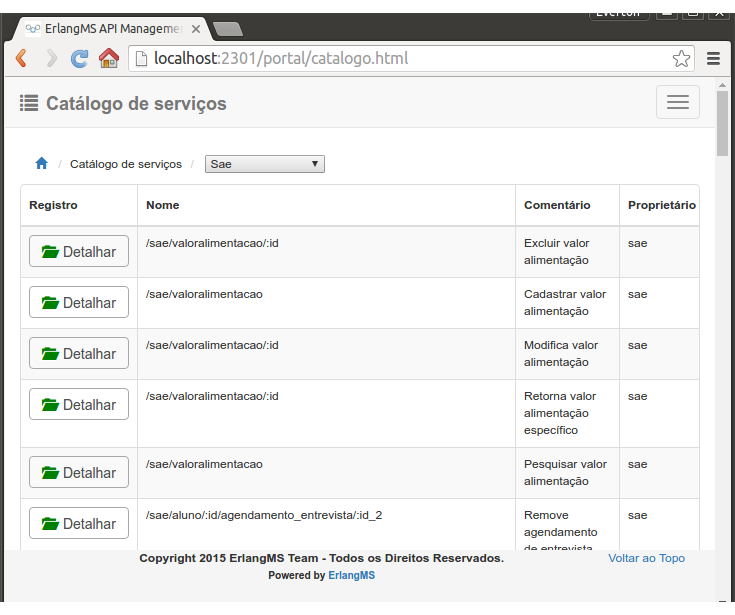
\includegraphics[scale=0.6]{img/processo/portal.png}
\caption{Lista dos serviços do projeto SAE no Portal de Serviços.}
\label{fig:portal_servicos}
\end{figure}






\subsection{Implementar os Serviços}

O desenvolvimento
dos serviços especificados
são realizados nesta atividade. Assim,
recomenda-se que os serviços estejam 
localizados dentro de um 
\emph{módulo de serviços} que representa 
um determinado domínio do negócio.
A Figura~\ref{fig:modulos_sae} apresenta
os 4 módulos
desenvolvidos no estudo de caso,
conectados ao barramento.



Para que os serviços possam ser implementados
em uma determinada linguagem (como o Java),
torna-se necessário um \acrfull{SDK}, que faz parte 
da arquitetura da abordagem. 
Embora o \acrshort{SDK} seja apresentado em mais detalhes na
Seção~\ref{arquitetura}, apenas para
reforçar, ele é um componente que conecta o módulo
ao barramento
e estabelece as bases da arquitetura proposta
para os módulos bem como possibilita
o envio e o recebimento
de mensagens entre os serviços de forma agnóstica.








\subsection{Deployment e Teste dos Serviços}

A granularidade da implantação que se propõe no processo
é por serviço.
Contudo, durante e após a implantação dos serviços, 
devem ser realizados os testes para verificar se 
os serviços funcionam corretamente.
Desse modo, o objetivo desta fase é
fazer o \textit{deployment}
e descobrir possíveis erros 
ou inconsistências
entre o que foi implementado
e o que está especificado
nos catálogos de serviços.


O \acrshort{SMSOC} propõem que 
os testes sejam automatizados
utilizando uma ferramenta 
que suporte uma abordagem \acrfull{BDD}
e, se possível, por equipes diferentes
para maximizar a descoberta de erros. 
De acordo com~\cite{solis2011study},
o \acrshort{BDD} é
uma filosofia onde o software
é construído de forma incremental e
guiado pelo comportamento esperado.
Assim, conforme investigado em~\cite{ragonha2013jasmine},
esta abordagem funciona bem com as 
práticas \acrshort{DDD}
adotadas neste processo
porque também trabalha com os conceitos de 
design centrado no domínio do negócio
sob uma perspectiva orientada às especificações.

Nesse contexto, 
para automatizar os testes
dos serviços 
desenvolvidos no 
projeto de modernização do \acrshort{SAE}, 
foi utilizado a ferramenta
de teste Jasmine.\footnote{A ferramenta de teste Jasmine está disponível
no sítio \url{http://jasmine.github.io}.} 
Apenas para ilustrar, a Figura \ref{fig:servicos_desenvolvidos}
lista um portal de teste da 
ferramenta Jasmine que possibilita
acompanhar a execução dos testes. Tais testes foram 
desenvolvidos com a linguagem Javascript.

\begin{figure}[htb]
\centering
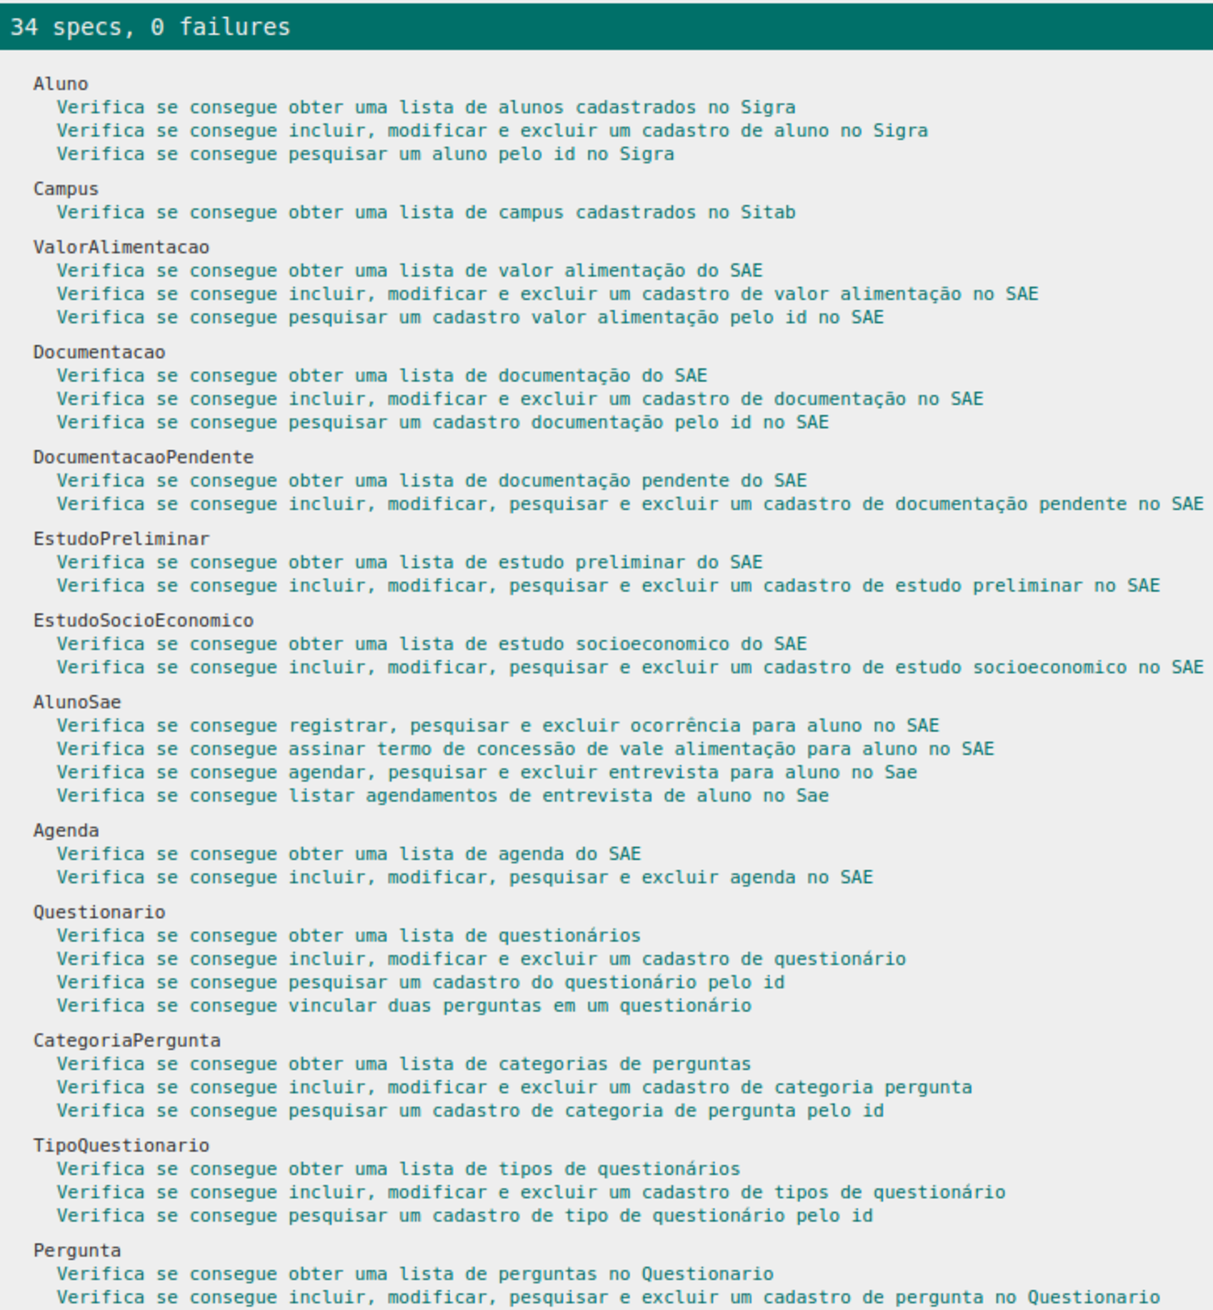
\includegraphics[scale=0.67]{/img/avaliacao/EstudoCaso/ServicosDesenvolvidos.pdf}
\caption{Lista de testes para os serviços desenvolvidos no SAE.}
\label{fig:servicos_desenvolvidos}
\end{figure}

\FloatBarrier

\begin{figure}[htb]
\centering
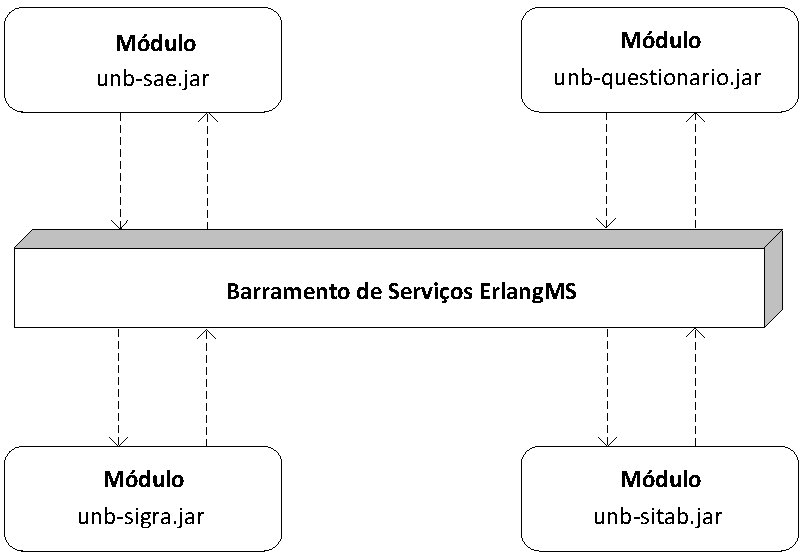
\includegraphics[scale=0.57]{img/processo/modulos_sae.pdf}
\caption{Módulos desenvolvidos para cada domínio do negócio do \acrshort{SAE}.}
\label{fig:modulos_sae}
\end{figure}

\FloatBarrier



\subsection{Front-end Design}

A abordagem proposta neste trabalho
envolve a modernização do sistema legado
através de uma arquitetura \acrshort{SOA},
onde o software é na verdade
um conjunto de serviços que 
são disponibilizados aos usuários
por meio de um barramento.

Sendo assim, para que os serviços possam ser 
acessados e consumidos
pelos usuários de uma forma simples,
torna-se necessário desenvolver a
interface visual para a aplicação, ou seja, o \textit{front-end}.
Note que, do ponto de vista dos usuários,
o \textit{front-end} é a parte do software
que o usuário vai interagir, 
sendo importante
disponibilizar uma interface amigável e intuitiva.

Embora o design do \textit{front-end} 
não seja o foco deste trabalho,
apenas para ilustrar o trabalho realizado
durante o estudo de caso, a Figura~\ref{fig:frontend}
mostra a interface visual do novo \acrshort{SAE}.
Esse \textit{front-end} está sendo desenvolvido usando 
Javascript e HTML5 em conjunto com as bibliotecas
de software Bootstrap\footnote{A biblioteca Bootstrap está disponível em http://getbootstrap.com.}, e jQuery\footnote{A biblioteca jQuery está 
disponível em https://jquery.com.}.

\begin{figure}[htb]
\centering
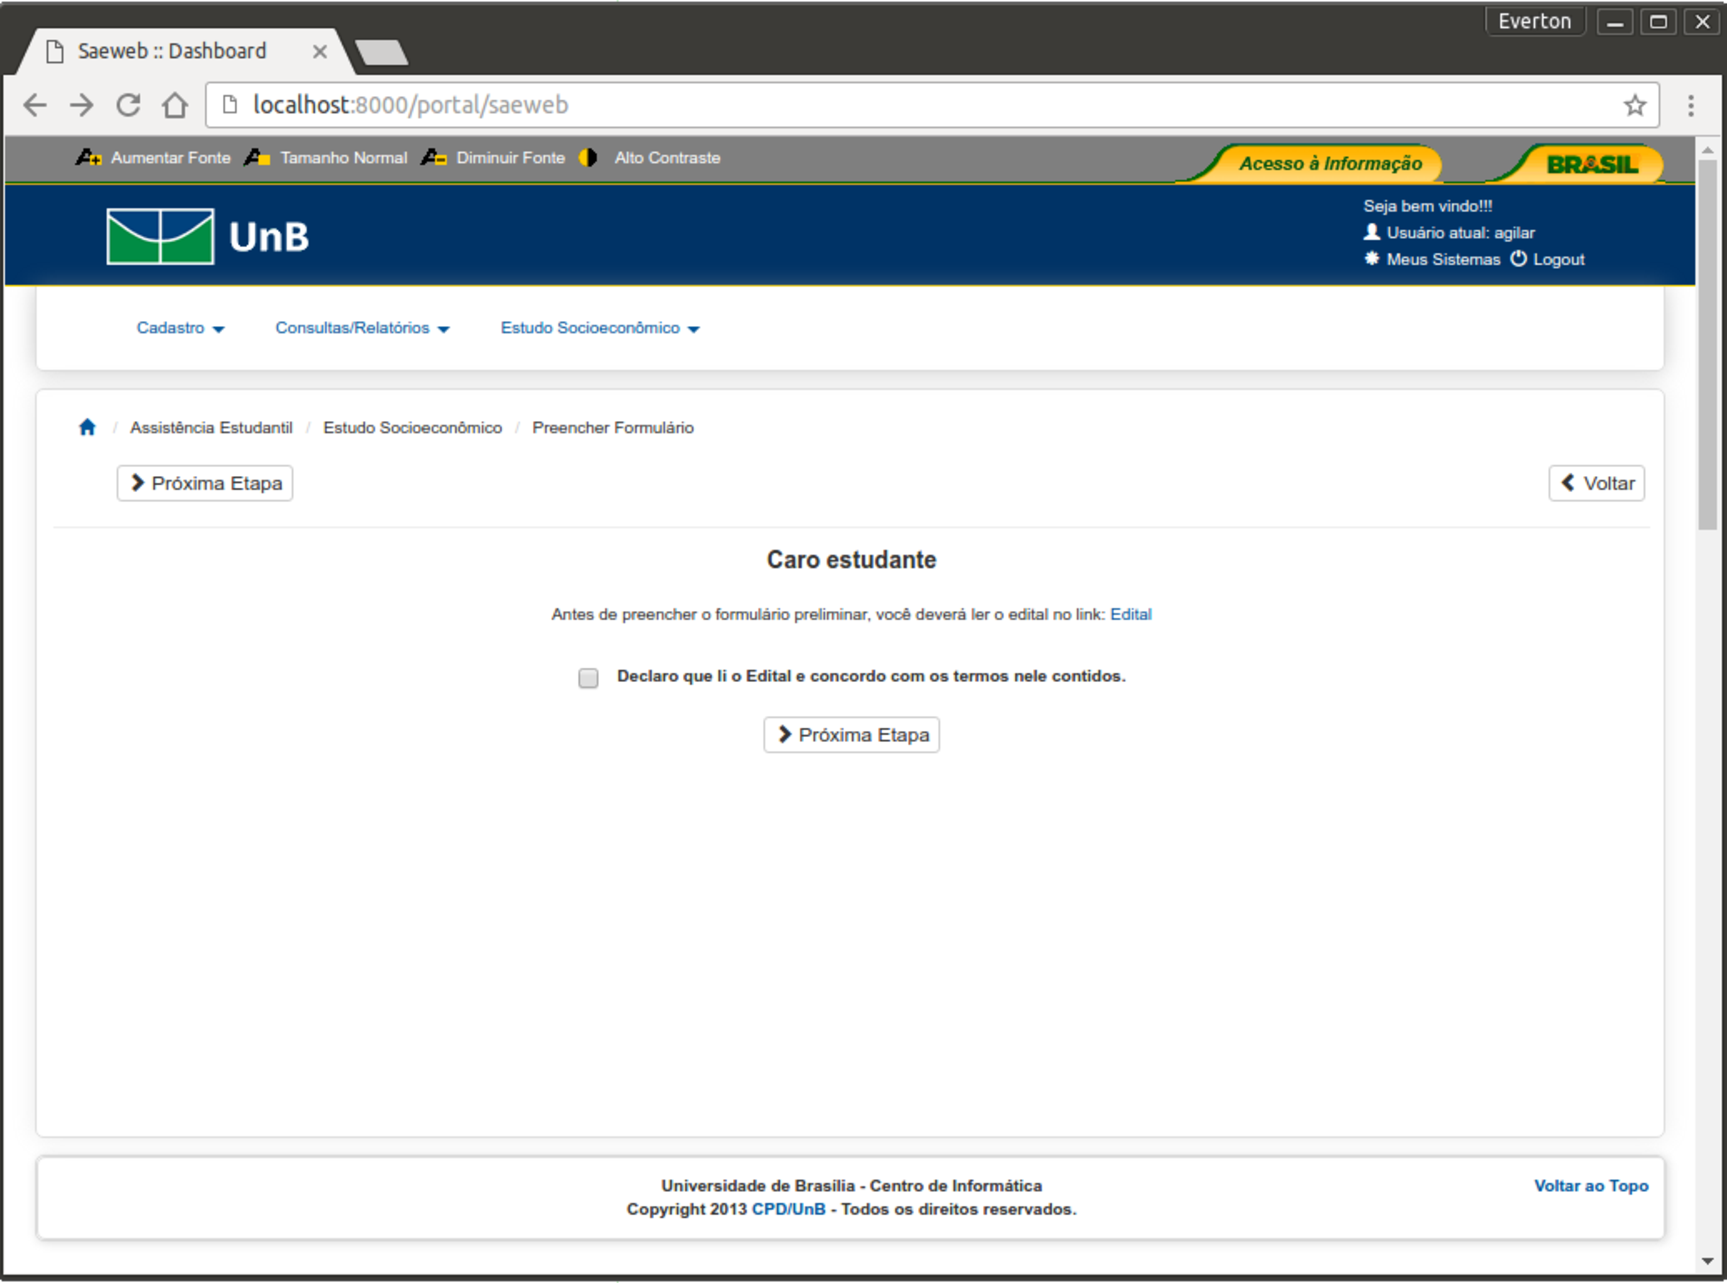
\includegraphics[scale=0.53]{/img/processo/saeweb.pdf}
\caption{Front-end desenvolvido para o sistema SAE.}
\label{fig:frontend}
\end{figure}
\FloatBarrier


\section{Arquitetura da Abordagem Proposta}\label{visao_geral}\label{arquitetura}

Diante da necessidade de conduzir a modernização dos sistemas legados na \acrshort{UnB},
optou-se por experimentar com a arquitetura orientada a servi\c cos, particularmente 
seguindo o estilo arquitetural \acrshort{REST}. 
Após estudos realizados pela equipe de analistas do CPD/UnB em 2014, em conjunto com os 
coordenadores das áreas de negócios da \acrshort{SSI}, a recomendação foi experimentar uma arquitetura 
\acrshort{SOA} para fazer a modernização dos sistemas legados, onde os sistemas novos e os legados poderiam coexistir e acessar os mesmos serviços. 

A abordagem proposta impõem o uso de um \acrfull{ESB} criado na 
linguagem funcional Erlang. O projeto 
está disponível no sítio \url{https://github.com/erlangms}
como pode ser visto na Figura~\ref{fig:erlangms_git} e conta com alguns colaboradores em seu desenvolvimento. De acordo com \cite{SOAPractice:2007}, um barramento permite 
a unificação do acesso aos serviços por meio de uma camada intermediadora.


\begin{figure}[htb]
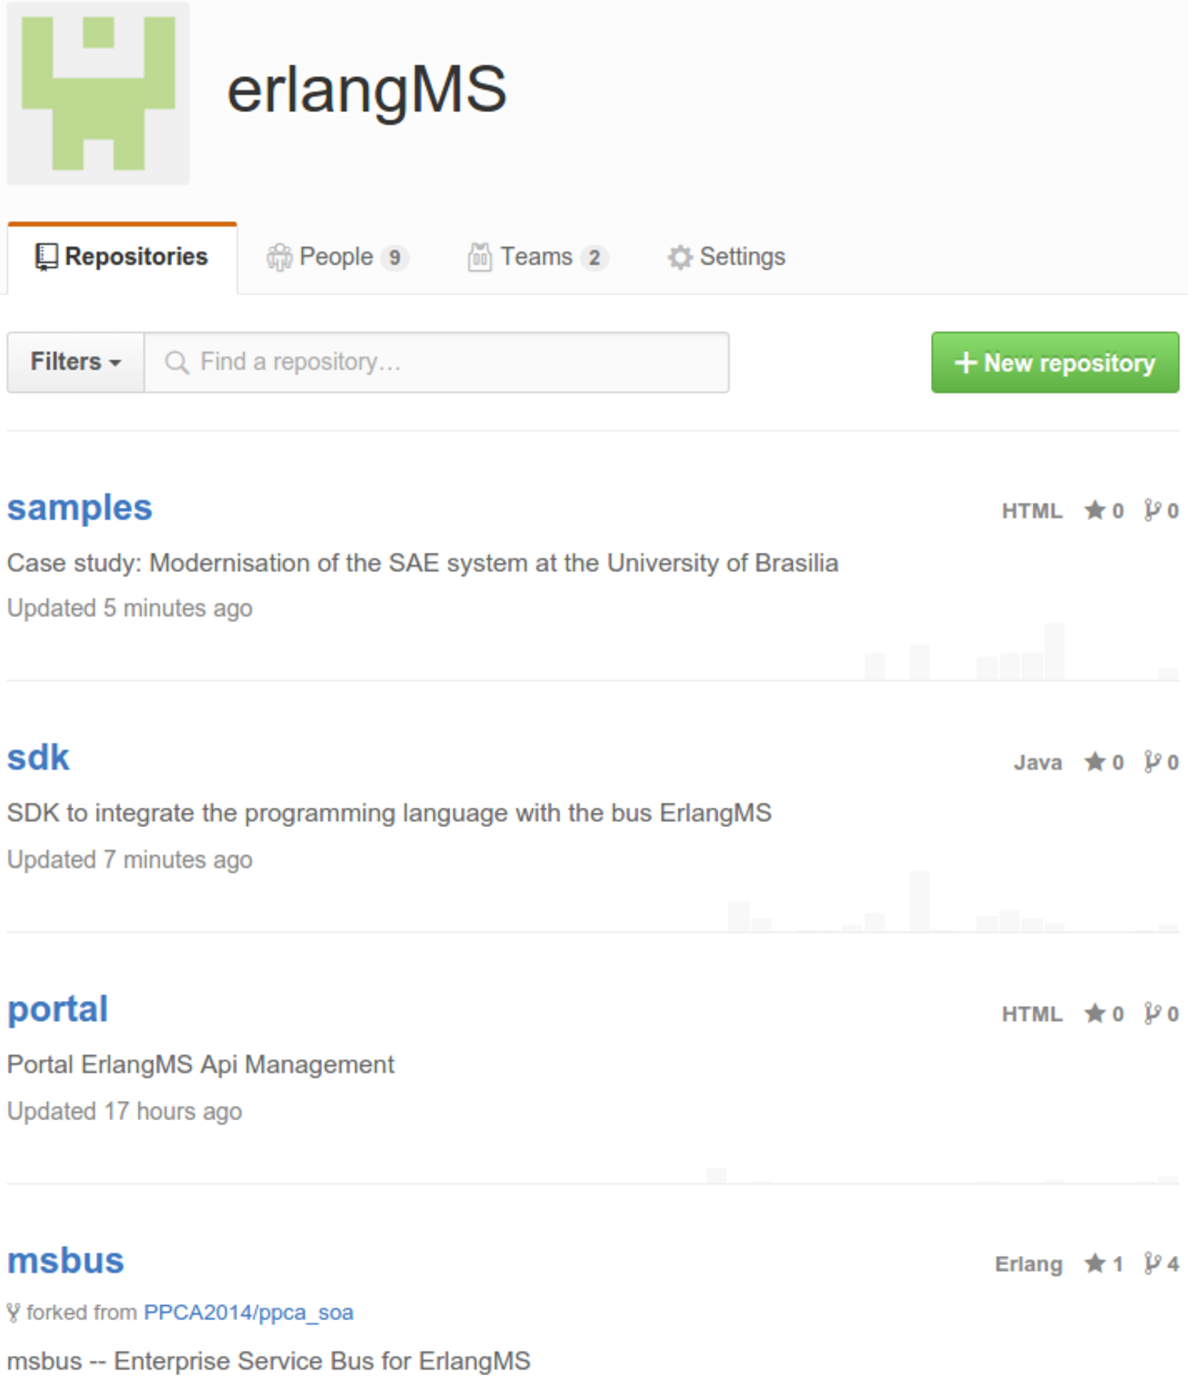
\includegraphics[scale=0.57]{/img/arquitetura/erlangms_git.pdf}
\caption{Sítio do projeto ErlangMS e da implementação do SAE.}
\label{fig:erlangms_git}
\end{figure}
\FloatBarrier



De acordo com a Figura~\ref{fig:arquitetura}, a arquitetura permite interligar os clientes aos serviços que contém as regras de negócios da organização. A implementa\c c\~{a}o de um novo 
barramento (em vez da ado\c c\~{a}o de um barramento pronto), permitiu obter
uma melhor compreens\~{a}o do estilo arquitetural \acrshort{REST} bem como o dom\'{i}nio de alguns 
elementos chave propostos na arquitetura, como o gerenciamento das requisições dos clientes e o catálogo de serviços. Além disso, possibilitou o emprego de uma solução que se mostrou simples, uma vez que a linguagem Erlang já disponibiliza bibliotecas de software para tratar requisições HTTP/REST e se comunicar com várias linguagens de programação.



A decisão de usar a linguagem Erlang na implementação do barramento 
ocorreu porque ela possui um ambiente de execução e um modelo de concorrência 
baseado em troca de mensagens entre atores integrados na própria linguagem que facilitam 
a construção de sistemas distribuídos escaláveis e tolerante a falhas. Nesse sentido, tanto os serviços em Erlang como os implementados em outra linguagem (como a linguagem Java), são vistos como atores, podendo receber e enviar mensagens de forma transparente e independente da sua localização.


\subsection{Design de Implementação dos Serviços}\label{design_implementacao}


O design de implementação dos serviços
proposto neste trabalho de dissertação é apenas uma recomendação de uso e
baseia-se fortemente 
nos padrões de design \acrshort{DDD} e \acrshort{SOA},
descritos em
~\cite{avram2007domain, evans2004domain, fowler2002patterns, krafzig2004service, SOA_patterns_2012}.
Para demonstrar o seu uso,
descreve-se a seguir 
a arquitetura de um módulo do \acrshort{SAE},
contendo
exemplos em código Java.\footnote{O código fonte completo 
da camada de serviços do sistema \acrshort{SAE} está disponível
no sítio \url{https://github.com/erlangms/samples/tree/master/sae/backend}.}.

A Figura~\ref{fig:arquitetura_modulo} ilustra
a anatomia de um módulo de serviços
de acordo com o padrão \textit{Service Layer}
descrito em~\cite{fowler2002patterns}.
A primeira observação que
se pode fazer é a 
organização interna sob uma arquitetura
em \textit{layers} (ou arquitetura em camadas),
cujo objetivo é separar os 
vários tipos de artefatos 
de um software de forma lógica e coesa~\cite{evans2004domain}.

O interessante deste design 
é a centralização dos códigos
que tem relação com o negócio da aplicação
em uma camada específica (a camada de serviços)
e o isolamento dos outros tipos
de artefatos, como a persistência dos dados, em outra camada,
o que pode, segundo~\cite{avram2007domain}, simplificar o desenvolvimento do sistema 
ao evitar (ou talvez minimizar) que diferentes tipos 
de códigos fiquem misturados.



\begin{figure}[htb]
\centering
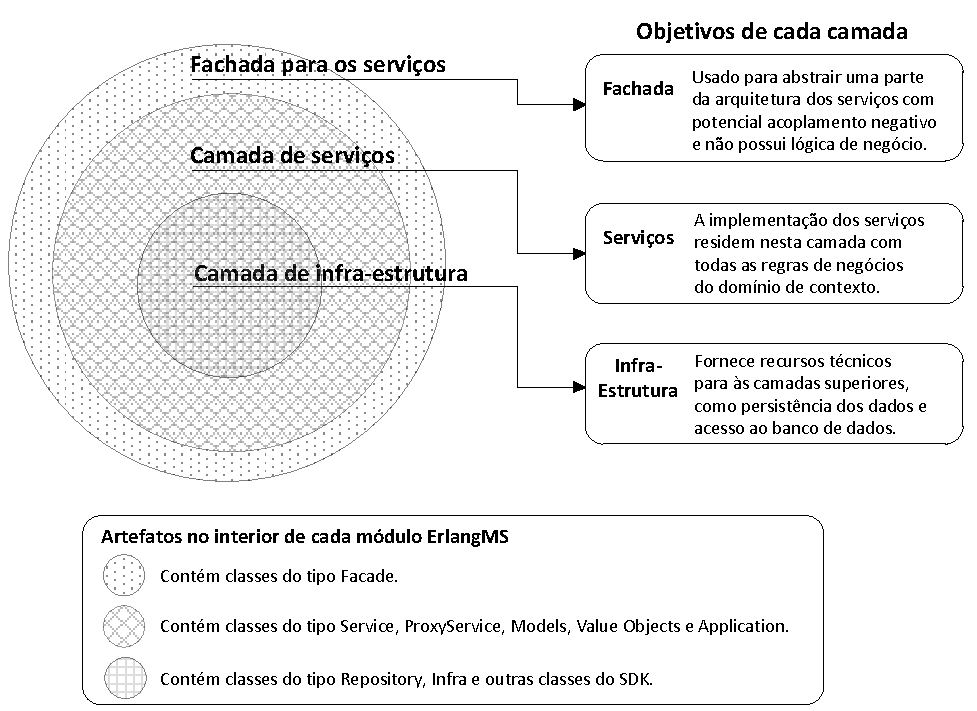
\includegraphics[scale=0.9]{img/processo/arquitetura_modulo.pdf}
\caption{Anatomia de um módulo da camada de serviços.}
\label{fig:arquitetura_modulo}
\end{figure}


Com base nestes aspectos, apresenta-se a seguir uma 
breve descrição da finalidade de cada camada,
no modelo de arquitetura proposto para 
os módulos de serviços.

\begin{itemize}

	\item Primeira Camada: De fachada.
	
	Implementa 
	o padrão \emph{ServiceFacade} 
	identificado em~\cite{SOA_patterns_2012}.
	Salienta-se que esta camada não deve 
	conter	lógica de negócio e 
	o seu objetivo é evitar 
	um possível acoplamento indesejado
	ao impedir que a lógica de negócio 
	localizada na camada de serviços
	seja exposta diretamente ao barramento.
	Assim, quando o cliente requisita um 
	serviço ao barramento,
	na verdade, é invocado um 
	método da fachada.

	Em termos práticos, a finalidade
	desta camada é possibilitar que 
	os parâmetros da requisição \acrshort{REST}
	sejam lidos e o método do serviço correspondente seja invocado
	com os dados que ele necessita. E, 
	no caso do serviço retornar
	uma resposta ao cliente, a fachada pode 
	realizar algum 
	processamento opcional (no estudo de caso não foi necessário)
	ou simplesmente retornar o 
	resultado ao cliente\footnote{O
	desenvolvedor não precisa preocupar-se 
	com a transformação dos dados de/e para \acrshort{JSON}, 
	isso é de responsabilidade do \acrshort{SDK} e do barramento.}.

	O Código~\ref{fig:exemplo_fachada} mostra um exemplo
	de fachada para o serviço \emph{QuestionarioService}
	do módulo unb\_questionario,
	onde há três métodos declarados que ao serem
	invocados, ocorrem os 
	seguintes eventos nessa ordem: 
	os dados da requisição
	são lidos a partir do \emph{IEmsRequest request}
	(interface que contém os dados da requisição); 
	após, é obtido a referência ao objeto \emph{QuestionarioApplication}, 
	responsável pelo acesso a camada de serviços do módulo; depois,
	a referência para o objeto do serviço correspondente é recuperada, 
	e finalmente; o método do serviço solicitado é invocado
	com os parâmetros requeridos.
	
	 
	
	
\lstset{language=Java,
        basicstyle=\footnotesize,
        numbers=left,
        numberstyle=\footnotesize,
        tabsize=2,
        numbers=none,
        rulesepcolor=\color{blue}}
             
\renewcommand{\lstlistingname}{Código}             
\begin{lstlisting}[caption=Exemplo de fachada para o serviço QuestionarioService., label=fig:exemplo_fachada] 

package br.unb.questionario.facade;

import br.unb.questionario.service.QuestionarioApplication;

public class QuestionarioFacade extends EmsServiceFacade {
	public Questionario findById(IEmsRequest request){
		Integer id = request.getParamAsInt("id");
		return QuestionarioApplication.getInstance()
			.getQuestionarioService()
			.findById(id);
	}
	
	public Questionario insert(IEmsRequest request){
		Questionario questionario = (Questionario) request.getObject(Questionario.class);
		return QuestionarioApplication.getInstance()
			.getQuestionarioService()
			.insert(questionario);
	}
	
	public boolean vinculaPerguntaAoQuestionario(IEmsRequest request){
		int questionario_id = request.getParamAsInt("id");
		int pergunta_id = request.getPropertyAsInt("pergunta");
		QuestionarioApplication.getInstance()
			.getQuestionarioService()
			.vinculaPerguntaAoQuestionario(questionario_id, pergunta_id);
		return true;
	}
	// outros métodos omitidos...
}
\end{lstlisting}
	
	
	\item Segunda Camada: De serviços.
	
	A camada de serviços consiste na parte mais 
	importante da arquitetura mostrada na Figura~\ref{fig:arquitetura_modulo}, 
	pois na visão de~\cite{evans2004domain, fowler2002patterns},
	é o local onde	concentra-se a lógica de domínio do negócio do sistema.
	Por conta disso, convém destacar que parte
	do foco do \acrshort{DDD},
	como identificado em~\cite{evans2004domain, fowler2002patterns}, 
	situa-se nessa camada, razão pela qual
	o design da arquitetura proposta
	tenta (na medida do possível) 
	não focar em tecnologia, 
	mas, em vez disso, entender as regras do negócio e
	como refleti-las no código fonte da aplicação 
	de maneira agnóstica.

	Nesse sentido, ao modelar a camada de serviços, 
	pode-se fazer uso de diversos \emph{blocos 
	de construção} definidos no \acrshort{DDD},
	que são, essencialmente, os artefatos que constituem
	esta camada. Para exemplificar e explicar 
	alguns conceitos desses artefatos, 
	segue uma descrição
	dos principais elementos utilizados na camada de serviços 
	dos módulos desenvolvidos no \acrshort{SAE}. 
	
	\begin{itemize}
	
		\item Entidades. São as classes de objetos que possuem 
						 identidade, comportamentos (ou métodos) 
						 e um ciclo de vida~\cite{evans2004domain}.
						 Por exemplo, 
						 um aluno do \acrshort{SAE}
						 que se autentica no sistema e realiza
						 a avaliação socioeconômica. Em sistemas Java 
						 típicos, como os desenvolvidos pelo CPD/UnB,
						 as classes de entidades podem 
						 ser comparados a classes \acrfull{POJO}, 
						 embora	um \acrshort{POJO} siga
						 algumas definições de design
						 que uma Entidade não precisa
						 (por exemplo,	ter um construtor padrão
						 sem argumentos e 
						 métodos \textit{getters} e \textit{setters}
						 para os atributos), 			 
						 de acordo com~\cite{kalin2013java}.


		\item \acrfull{VO}. São as classes de objetos
						que são modeladas geralmente para 
						carregar dados e
						possuem o sufixo \emph{Vo}
						no \acrshort{SAE} por convenção.
						Uma classe desse tipo é o
						\emph{CampusVo} que
						possui apenas dois atributos (id e nome)
						e foi implementada para que os serviços 
						do módulo unb\_sae possam carregar a 
						lista de campus a partir de um serviço
						que está no módulo unb\_sitab. Existem
						outras características sobre \acrshort{VO}
						que não serão tratadas aqui por simplicidade
						mas em~\cite{fowler2002patterns} 
						é discutido em mais detalhes.
						
						

		\item \textit{Factory}. São as classes responsáveis
			por \emph{fabricar} os objetos e usadas
			na fabricação dos serviços nessa camada. 
			Essas classes tem 
			o sufixo \emph{Application} por convenção 
			(QuestionarioApplication, por exemplo)
			e apenas por curiosidade, classes desse tipo
			são também conhecidas pelo padrão
			\textit{ApplicationService} no guia de padrões
			de design Java EE (Core J2EE
			Patterns)~\cite{alur2003core}.
			
			Como é possível
			observar no Código~\ref{fig:exemplo_fachada} de exemplo,
			a fachada somente acessa um objeto de
			serviço mediante o QuestionarioApplication. 
			O principal motivo
			para o uso desse design
			no \acrshort{SAE} é esconder 
			a forma como se criam ou
			injetam os objetos (com injeção de dependência),
			uma vez que é desejável que o \acrshort{SDK}
			em outras linguagens de programação
			façam o mesmo,
			independente da tecnologia empregada para isso.
			Outro motivo importante é minimizar
			as dependências e o acoplamento entre os objetos. 
			Note que isso foi obtido, pois,
			é possível verificar que os métodos 
			da fachada acessam somente a interface 
			do serviço e não precisam importar 
			a classe de implementação do serviço,
			somente a classe QuestionarioApplication
			em br.unb.questionario.service.
		
		\item \textit{Services}. São as classes que contém 
				as regras de negócios da aplicação e
				a implementação do serviço
				de acordo com a sua especificação 
				no catálogo de serviços do projeto.
				Note que os objetos do tipo Entidades
				também contém regras de negócios
				porque o \acrshort{DDD} trabalha com objetos 
				com comportamentos 
				e não somente atributos (ou seja, objetivos não anêmicos).
				
				Além disso, uma observação importante
				sobre os serviços identificado em~\cite{fielding1999rfc},
				é que as classes de serviço não devem ter estado,
				obedecendo dessa forma, a restrição REST \textit{Stateless},
				discutida no Capítulo~\ref{fundamentos}.
	\end{itemize}
	
	Para finalizar a descrição dos conceitos discutidos 
	sobre a camada de serviços da arquitetura proposta,	
	o Código~\ref{fig:exemplo_servico} mostra a implementação 
	parcial do código fonte da classe do 
	serviço QuestionarioService com os 3 métodos invocados
	pela fachada demonstrada anteriormente 
	no Código~\ref{fig:exemplo_fachada}. Perceba que 
	o serviço faz uso da camada de infraestrutura apresentada a seguir.
	
	
\lstset{language=Java,
        basicstyle=\footnotesize,
        numbers=left,
        numberstyle=\footnotesize,
        tabsize=2,
        numbers=none,
        rulesepcolor=\color{blue}}
             
\renewcommand{\lstlistingname}{Código}             
\begin{lstlisting}[caption=Exemplo de implementação do serviço QuestionarioService., label=fig:exemplo_servico]

package br.unb.questionario.service;

// imports omitidos para facilitar a visualização

public class QuestionarioService {
	public Questionario findById(Integer id) {
		return QuestionarioInfra.getInstance()
			.getQuestionarioRepository()
			.findById(id);
	}
	
	public Questionario insert(Questionario questionario) {
		questionario.validar();
		return QuestionarioInfra.getInstance()
			.getQuestionarioRepository()
			.insert(questionario);
	}	
	
	public void vinculaPerguntaAoQuestionario(
		int questionario_id, int pergunta_id) {
		Questionario questionario = findById(questionario_id);
		Pergunta pergunta = QuestionarioApplication.getInstance()
								.getPerguntaService()
								.findById(pergunta_id);
		questionario.vinculaPergunta(pergunta);
	}	
	// outros métodos omitidos...
}
\end{lstlisting}
	



	\item Terceira Camada: Infraestrutura.

		É muito comum, parte do software 
		não estar diretamente relacionado 
		ao domínio do negócio, 
		mas a sua infraestrutura de apoio~\cite{avram2007domain}.
		Assim, a finalidade desta camada
		é prover os recursos técnicos
		necessários para as
		camadas superiores do módulo, 
		como o acesso, a persistência
		e a consulta dos objetos em um banco de dados, 
		a escrita de logs para o registro de eventos relevantes,	
		entre outros recursos.

		No entanto,~\cite{evans2004domain, fowler2002patterns} 
		afirmam que esta camada 
		deve prover os recursos 
		tecnológicos de forma isolada,
		não expondo
		os detalhes internos da 
		infraestrutura,
		pois podem comprometer a 
		camada de serviços
		com aspectos
		técnicos do software misturados com
		as regras de negócios. 
		Nesse caso,~\cite{avram2007domain} 
		sugere que a camada de infraestrutura
		seja exposta através de interfaces simples.
	

		Assim como na camada de serviços,
		existem alguns artefatos
		para modelar esta camada, 
		previstos no \acrshort{DDD}~\cite{evans2004domain}.
		Na arquitetura proposta, 
		sugere-se utilizar
		os artefatos \textit{Repository} (Repositório)
	 	e o \textit{Factory}, para lidar
	 	com os desafios discutidos anteriormente.
		Segue uma breve descrição
		de alguns conceitos desses artefatos 
		com exemplos de utilização em código Java.
			
		\begin{itemize}
		
			\item \textit{Repository}.	Tradicionalmente, a maioria das aplicações
			precisam persistir ou recuperar os objetos 
			em algum banco de dados.
			Sendo assim, o objetivo das 	
			classes \textit{Repository} é
			basicamente gerenciar o ciclo de vida dos objetos, 
			como as Entidades ou \acrshort{VO},
			centralizando as 
			operações de criação, modificação, exclusão
			e consulta de objetos em um banco de dados~\cite{vernon2013implementing}.
			
			Para exemplificar,
			o Código~\ref{fig:exemplo_repository} mostra
			a classe de repositório \emph{OcorrenciaRepository} 
			do módulo \emph{unb\_sae}, 
			cujo objetivo é gerenciar o ciclo de vida das
			ocorrências de um estudante, 
			um tipo
			de evento ocorrido em um determinado período	 
			que pode acarretar na suspensão do
			auxílio alimentação,
			mediante justificativa, de acordo 
			com as normas do \acrfull{PNAES}. 
			As classes \textit{Repository}
			na arquitetura proposta possuem
			o sufixo Repository por convenção. 
			
			A primeira observação 
			nessa classe é quanto 
			a sua interface. 
			Por motivos já discutidos,
			as classes \textit{Repository}
			foram projetadas para
			terem uma interface simples. 
			Note que
			a classe OcorrenciaRepository 
			herda de 
			\textit{EmsRepository} (veja a Figura~\ref{fig:diagrama_classe_ems_repository})
			fornecido pelo \acrshort{SDK}
			e não precisa implementar nenhum 
			método público nesse exemplo, 
			uma vez que as operações 
			herdadas são suficientes. Em outras classes,
			poderá ser necessária a criação
			de outros métodos públicos conforme 
			a necessidade. Pode-se notar também
			alguns métodos protegidos
			e que na implementação em Java do \acrshort{SDK}, 
			os repositórios usam o \acrfull{JPA},
			um \textit{framework} de persistência de dados.
			Este é um detalhe técnico que importa
			somente aos repositórios e não devem 
			ser expostos, como 
			verificou-se em~\cite{evans2004domain, fowler2002patterns}.			
			Por curiosidade, o diagrama de classe 
			na Figura~\ref{fig:diagrama_classe_ems_repository}
			exibe as operações comuns a todas
			as classes \textit{Repository}
			na arquitetura.
		
		
\begin{figure}[htb]
\centering
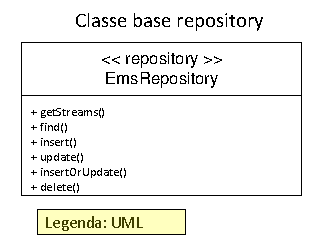
\includegraphics[scale=1.5]{img/processo/exemplo_classe_repository.pdf}
\caption{Classe base repository.}
\label{fig:diagrama_classe_ems_repository}
\end{figure}
\FloatBarrier
	
	

	


			Como pode-se ver na Figura~\ref{fig:diagrama_classe_ems_repository},
			há uma operação denominada \textit{getStreams()}, 
			que	merece uma explicação. A ideia
			desse método surgiu 
			no estudo de caso (não fazia parte 
			da proposta inicial da arquitetura) 
			para
			fornecer uma 
			interface comum para 
			consulta de objetos.
			Ou seja,
			como a maioria das operações 
			geralmente são consultas (nos sistemas do CPD/UnB),
			buscou-se uma forma de expor uma 
			pequena \acrshort{API}
			para que o desenvolvedor não
			precise 
			implementar um novo método 
			de consulta sempre que for 
			necessário 
			pesquisar objetos por 
			determinada 
			condição (contando que a pesquisa seja simples).
			O Código~\ref{fig:exemplo_get_stream} ilustra o uso 
			desta \acrshort{API} em alguns
			métodos da entidade Aluno fazendo uso 
			do método \textit{getStreams()},
			onde é possível notar uma certa praticidade
			com o uso desta funcionalidade,
			além de possibilitar emitir as consultas
			usando uma linguagem tipificada
			em vez de usar as linguagens de consultas
			tradicionais, como a \acrfull{SQL}.
			
		
			\item \textit{Factory}. São as classes responsáveis
			por fabricar os 
			repositórios (ou outros objetos)
			da camada de infraestrutura, 
			tendo por convenção,
			o sufixo \emph{Infra} neste trabalho.
			No Código~\ref{fig:exemplo_get_stream},
			é possível observar 
			que a classe Aluno
			acessa os repositórios requeridos
			por meio da classe \emph{SaeInfra}, 
			o \textit{Factory} da camada de 
			infraestrutura
			do módulo unb\_sae. 
			O principal 
			motivo do uso desse design,
			como discutido anteriormente,
			é esconder a forma como se criam
			os objetos.
		
		\end{itemize}


\end{itemize}




\lstset{language=Java,
        basicstyle=\footnotesize,
        numbers=left,
        numberstyle=\footnotesize,
        tabsize=2,
        numbers=none,
        rulesepcolor=\color{blue}}
             
\renewcommand{\lstlistingname}{Código}             
\begin{lstlisting}[caption=Exemplo de implementação do repositório QuestionarioRepository., label=fig:exemplo_repository]
package br.unb.sae.infra;

// imports omitidos para facilitar a visualização

public class OcorrenciaRepository extends EmsRepository<Ocorrencia>{
	
	@PersistenceContext(unitName = "service_context")
	protected EntityManager saeContext;
	
	@Override
	protected Class<Ocorrencia> getClassOfModel() {
		return Ocorrencia.class;
	}

	@Override
	protected EntityManager getEntityManager() {
		return saeContext;
	}

}
\end{lstlisting}


\lstset{language=Java,
        basicstyle=\footnotesize,
        numbers=left,
        numberstyle=\footnotesize,
        tabsize=2,
        numbers=none,
        rulesepcolor=\color{blue}}
             
\renewcommand{\lstlistingname}{Código}             
\begin{lstlisting}[caption=Exemplo de uso do método getStream() dos repositórios para consulta., label=fig:exemplo_get_stream]
package br.unb.sae.model;

// imports omitidos para facilitar a visualização

public class Aluno{

	private boolean assinouTermoConcessaoValeAlimentacao(
		String periodo) {
			int this_aluno = getId();
			return SaeInfra.getInstance()
				.getAssinaturaTermoBaRepository()
				.getStreams()
				.anyMatch(a -> a.getAluno() == this_aluno &&
							    a.getPeriodo().equals(periodo));
	}

	private boolean existeOcorrenciaAberto(
		String periodo, Date dataInicio) {
			int this_aluno = getId();
			return SaeInfra.getInstance()
				.getOcorrenciaRepository()
				.getStreams()
				.anyMatch(a -> a.getAluno() == this_aluno &&
							   a.getPeriodo().equals(periodo) &&
					       a.getDataInicio().equals(dataInicio));
	}

	public List<Ocorrencia> getListaOcorrencia() {
		int aluno_id = getId();
		return SaeInfra.getInstance()
				.getOcorrenciaRepository()
				.getStreams()
				.where(a -> a.getAluno() == aluno_id)
				.toList();
	}    
	
	public Ocorrencia findOcorrenciaById(Integer idOcorrencia) {
		return SaeInfra.getInstance()
			.getOcorrenciaRepository()
			.findById(idOcorrencia);
	}
	
	public List<AssinaturaTermoBa> getListaAssinaturaTermoConcessaoValeAlimentacao() {
		int this_aluno = getId();
		return SaeInfra.getInstance()
				.getAssinaturaTermoBaRepository()
				.getStreams()
				.where(a -> a.getAluno() == this_aluno)
				.toList();
	}
	// outros métodos omitidos
}
\end{lstlisting}



\subsection{Roteamento das Mensagens}\label{roteamento}

A arquitetura segue o conceito de \acrfull{SOC}, 
um paradigma que promove a composição de serviços \emph{em uma rede de serviços} 
fracamente acoplados, com o objetivo de criar processos de negócio dinâmicos 
e flexíveis através da interconexão de sistemas computacionais~\cite{SOAIntBlueprint:2010}. 

Dessa forma, o barramento suporta a mediação, roteamento, 
transformação de dados e a orquestração dos serviços. Para isso, adotou-se o 
estilo arquitetural \acrshort{REST} e o formato \acrshort{JSON} para o envio e 
recebimento das mensagens do cliente. Essa restrição de design teve o 
objetivo de facilitar a 
implementação do barramento. 

Na verdade, o esquema de comunicação da arquitetura ocorre por meio de 
duas vias distintas, como ilustra a Figura~\ref{fig:roteamento_mensagens}: Na primeira via, 
existe a comunicação do cliente para 
consumir algum serviço no barramento. Essa comunicação é via uma 
interface \acrshort{REST}, razão pela qual o cliente (que pode ser qualquer sistema, 
independente da sua linguagem de programação ou plataforma) 
precisa suportar chamadas de serviços em \acrshort{REST}. Na segunda via, tem a comunicação 
do barramento com o serviço, que está implementado em 
alguma linguagem de programação (Erlang, Java, etc.). Essa comunicação dá-se via
sistema de mensageria disponível
em Erlang que possibilita uma comunicação assíncrona 
com várias linguagens de programação de forma muito rápida por trafegar os dados 
no formato binário e com baixa latência na rede\cite{Armstrong:2013:PES:2566708}.

Assim, a função do barramento é rotear as requisições \acrshort{REST} para algum serviço processar 
e devolver o resultado de volta para o cliente, como ilustra a Figura~\ref{fig:arquitetura}. Este roteamento é possível porque o Erlang e seu ambiente de execução, permitem identificar quais serviços estão operando de forma transparente, sejam processos Erlang nativos ou processos de outra linguagem de programação suportada. 

\begin{figure}[htb]
\centering
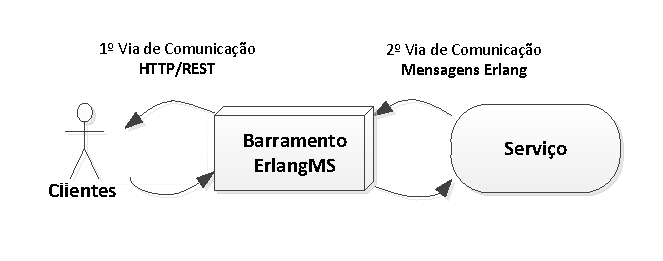
\includegraphics[scale=1.2]{/img/arquitetura/roteamento_mensagens.pdf}
\caption{Esquema do roteamento das mensagens da arquitetura.}
\label{fig:roteamento_mensagens}
\end{figure}
\FloatBarrier



\subsection{Linguagens de Programação Suportadas}\label{ling_suportada}

Potencialmente, qualquer linguagem pode ser utilizada para implementar os 
serviços nessa arquitetura, sendo que, o CPD/UnB vai utilizar a linguagem Java 
por ser de relativo domínio pelos membros da \acrshort{SSI} e já existir artefatos 
implementados nessa linguagem que poderão ser transformados em serviços, 
como a autenticação e o controle de acesso dos usuários aos sistemas da \acrshort{UnB}. A
arquitetura também suporta a linguagem Erlang para implementar os serviços, sendo esta
de forma nativa.

Para desenvolver os serviços em uma determinada linguagem de programação, 
torna-se necessário um \acrfull{SDK} para integrar a linguagem ao barramento de serviços. Neste trabalho, foi disponibilizado o \acrshort{SDK} \emph{ems\_java} para integrar
a linguagem Java ao barramento de serviços, como mostra a Figura~\ref{fig:erlangms_git}. 
Já está em desenvolvimento
o \acrshort{SDK} \emph{ems\_net} para 
integrar as linguagens C\# e VB.Net,
por um aluno de graduação
da \acrshort{UnB}
que participou do estudo de caso (Capítulo \ref{avaliacao}).



\subsection{Modelo de Computação Assíncrona}\label{modelo_computacao}

A arquitetura dá ênfase para um modelo de 
computação assíncrona onde os clientes não precisam ficar aguardando 
as solicitações de serviços. Na especificação do catálogo de serviços,
existe um atributo que indica se o processamento do serviço
pode ser assíncrono (atributo async).


Para se ter uma ideia da importância deste recurso para o CPD/UnB, existem algumas
rotinas de negócios processadas em lote que levam muito tempo para serem executadas, como o processamento 
das matrículas no sistema \acrshort{SIGRA} (executada durante as fases 
de pré-matrícula e matrícula dos estudantes), o lançamento das notas dos 
estudantes no sistema MatriculaWeb (executada nos finais de semana), o cálculo 
do grupo vigente das pessoas
que tem direito ao Restaurante Universitário (executada todos os 
dias durante o período noturno para determinar qual será o custo do vale alimentação), entre outros. 

Nesse contexto, a ideia é que se possa ter um catálogo de serviços com esses 
serviços documentados e que o 
barramento gerencie a execução 
desse tipo de serviço, notificando o responsável quando a 
requisição estiver concluída. Atualmente, o sucesso ou falha da execução 
dessas rotinas no CPD/UnB são verificadas manualmente consultando as tabelas do banco de dados.


\subsection{Cluster de Serviços}\label{cluster_servico}


A arquitetura permite que os serviços possam ser replicados em vários \textit{nodes}. Um \textit{node} é um aglomerado de serviços que são identificados por um nome lógico, sendo que o conjunto de nodes representa
um \textit{cluster} de serviços.

Nessa arquitetura, recomenda-se ter vários \textit{nodes} para evitar os possíveis pontos únicos de falhas. Tal estratégia permite que, caso um servidor/serviço apresente falha e pare de responder, o serviço continue \textit{online} enquanto existir outros \textit{nodes} funcionando com a implementação do serviço publicado no barramento. 

Além disso, no caso do CPD/UnB, por exemplo, por terem escolhido a linguagem Java, os serviços implementados 
serão empacotados em pacotes \emph{Java EE} e publicados nos servidores de aplicação JBoss (que são nodes, cada um com um nome único).
Assim, essas instâncias JBoss são vistas como \textit{nodes} que contém a implementação de um ou mais serviços
que foram disponibilizados no catálogo de serviços do barramento.

Ressalta-se que o barramento também é um node no \textit{cluster} e os módulos 
internos do barramento agem como serviços. Como pode-se ver na Figura~\ref{fig:arquitetura}, alguns dos 
principais serviços do barramento são o \emph{Server HTTP}, o módulo que faz o parser das mensagens HTTP/REST; o \emph{Dispatcher}, que faz o despacho das requisições para o serviço correspondente e; o \emph{Catalogo} que gerencia o catálogo de serviços. 

Por fim, sendo o barramento também um node, admite-se mais de uma instância em execução para evitar os pontos únicos de falhas no acesso ao barramento. Nesse caso, será necessário a utilização de um software 
do tipo balanceador de carga para distribuir as requisições para os serviços
entre as instâncias do barramento.




\subsection{Catálogo de Serviços}\label{catalogo_serviços}

Um componente chave é o catálogo de serviços, 
que em linhas gerais, dá visibilidade aos serviços 
disponibilizados, permitindo a reusabilidade dos componentes de software, 
uma vez que, estando o serviço publicado no barramento de serviços (conforme
a arquitetura vista na Figura~\ref{fig:arquitetura}), ele poderá ser 
acessado por diversas outras aplicações, inclusive aquelas que não
estavam previstas inicialmente. 

Nesse sentido, o catálogo de serviço está sendo concebido para ser administrado a partir 
de arquivos em formato \acrshort{JSON} e futuramente por
meio de um \emph{Portal Web}, já desenvolvido 
de forma preliminar para o projeto. 

A definição do catálogo inclui metadados para descrever os serviços oferecidos
de acordo com o modelo descrito por~\cite{OASISRefArch:2012}, a qual 
contém informações como o nome e descrição do serviço, o responsável pelo serviço, 
a \acrshort{URL}, os parâmetros do serviço, o tipo de autenticação, 
se o serviço é assíncrono, entre outros dados importantes. 
Para exemplificar, a especificação demonstrada
no Código~\ref{fig:catalogo_processo} mostra 
a definição do catálogo de alguns serviços para o \acrfull{SAE} da \acrshort{UnB}.



\subsection{Outros Requisitos Funcionais e Não Funcionais}\label{outros_req}

A seguir, apresenta-se alguns outros requisitos funcionais e não funcionais da arquitetura:

\begin{enumerate}[(RQ1)]

\item Prover uma interface RESTful para comunicação com os clientes. A comunicação 
entre o cliente e o barramento será por meio de uma \acrshort{API} \acrshort{REST}, 
suportando o subconjunto de operações \acrshort{HTTP} \textit{GET, POST, PUT e DELETE}. 
O objetivo \'{e} fornecer uma tecnologia agnóstica sobre a linguagem de programa\c c\~{a}o
para troca de mensagens. Cada requisição deverá conter toda informação do 
pedido e nenhum estado das comunicações entre as mensagens deverá ser mantido. 
Além disso, cada recurso será unicamente direcionado através da sua \acrshort{URI}.


\item Escalabilidade e tolerância a falhas (Requisito não funcional). Deve ser
escalável (suportar uma carga de trabalho maior quando necessário) e recuperar-se
de possíveis falhas no processamento das solicitações. Além disso, 
uma requisição a um serviço de longa duração não deve comprometer o processamento 
das demais solicitações e qualquer falha no atendimento deverá retornar ao cliente 
na forma de uma mensagem \acrshort{JSON} descrevendo o motivo do erro.


\item Monitoramento dos serviços publicados. O barramento deverá prover um portal de 
gerenciamento onde será possível monitorar o consumo dos serviços utilizados e 
listar os serviços disponíveis no catálogo para uso.

\end{enumerate}



\subsection{Histórico de Desenvolvimento do Barramento}\label{historico_barramento}

O projeto do barramento de serviços, denominado \emph{ErlangMS}, 
teve início na disciplina de \textit{Construção de Software} do Mestrado
Profissional em Computação Aplicada, da \acrlong{UnB}, através de 
aulas práticas e seminários. 

No primeiro seminário da disciplina, apresentou-se o 
protótipo do módulo HTTP desenvolvido para 
suportar a interface de comunicação \acrshort{REST}. Após, 
com a implementação desse módulo, o próximo passo foi desenvolver o módulo de
roteamento das requisições (o módulo \textit{Dispatcher}). Como não 
existia ainda um \emph{catálogo de serviço}, as rotas dos serviços 
foram inseridas diretamente no código fonte. Dois módulos de serviços foram criados 
para testar o roteamento preliminar: o serviço que trata a \acrshort{URL} ‘‘/‘‘ e responde com a 
mensagem \{‘‘\textit{message}‘‘: ‘‘\textit{It works}‘‘\} e o serviço que trata 
a \acrshort{URL} ‘‘/\textit{hello}\_\textit{world}‘‘ e retorna a 
mensagem \{‘‘\textit{message}‘‘: ‘‘Ola mundo‘‘\}.

Posteriormente, com a arquitetura do barramento definida, o código fonte
do projeto foi refatorado com os princípios de design da \acrfull{OTP}, 
o \textit{framework} da linguagem Erlang para construção 
de aplicações escaláveis e tolerante a falhas.

A partir disso, implementou-se o catálogo de serviços (a partir 
da leitura de um arquivo \acrshort{JSON}), tendo
o módulo \textit{Dispatcher} sido reescrito para localizar
os serviços nesse catálogo (a partir da \acrshort{URL} e do método
\acrshort{HTTP} da requisição) para redirecionar a requisição
para o serviço correspondente. Nesse trabalho de implementação, incluiu-se 
suporte para a transformação dos dados de/para \acrshort{JSON} (de
forma transparente dos processos de serviços) e 
o suporte para o tratamento dos erros \acrshort{HTTP} mais comuns. 

O próximo passo foi incluir alguns recursos de tolerância a falhas 
no barramento de serviços. Assim, foi incluído suporte 
para a supervisão de processos da \acrshort{OTP} (processos que
supervisionam outros processos filhos) para monitorar os módulos
do barramento e permitir a sua recuperação em caso de falha.

Apenas para ilustrar, a Figura~\ref{fig:instancia_barramento} mostra
a interface em linha de comando de uma instância do
barramento ErlangMS executando em um servidor Linux. Salienta-se que
o projeto do barramento é multiplataforma e 
pode ser executado também nos sistemas operacionais
Windows e Mac.

\begin{figure}[htb]
\centering
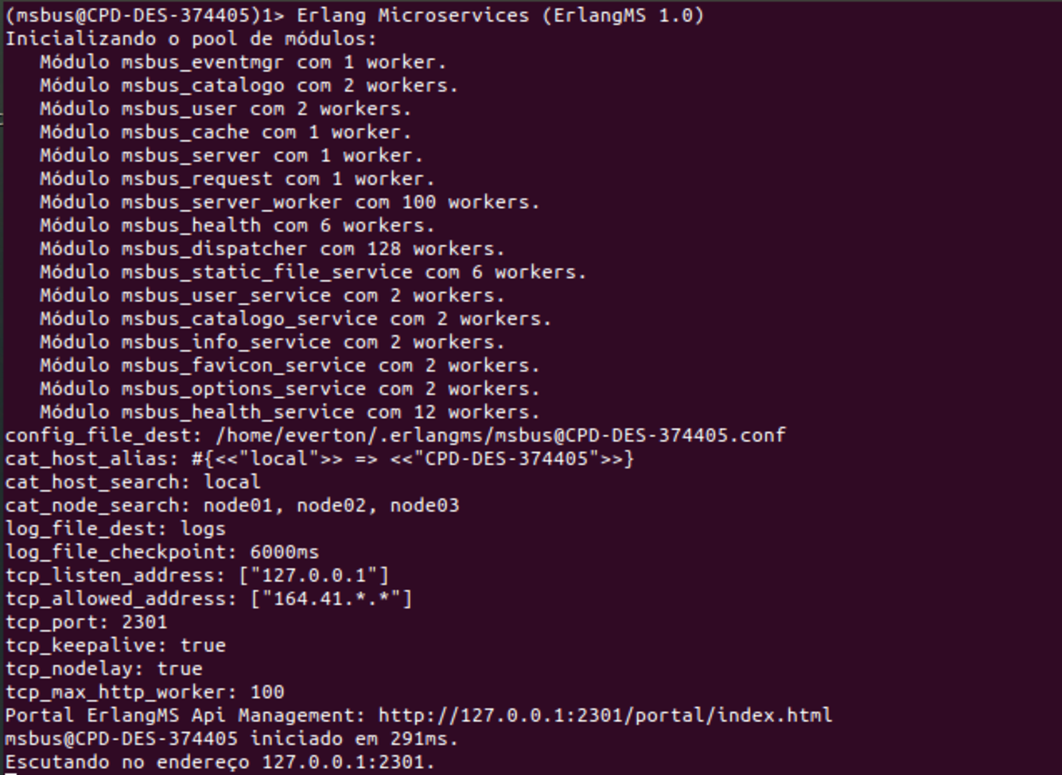
\includegraphics[scale=0.87]{img/arquitetura/instancia_barramento.pdf}
\caption{Interface em linha de comando do barramento ErlangMS.}
\label{fig:instancia_barramento}
\end{figure}






\begin{figure}[htb]
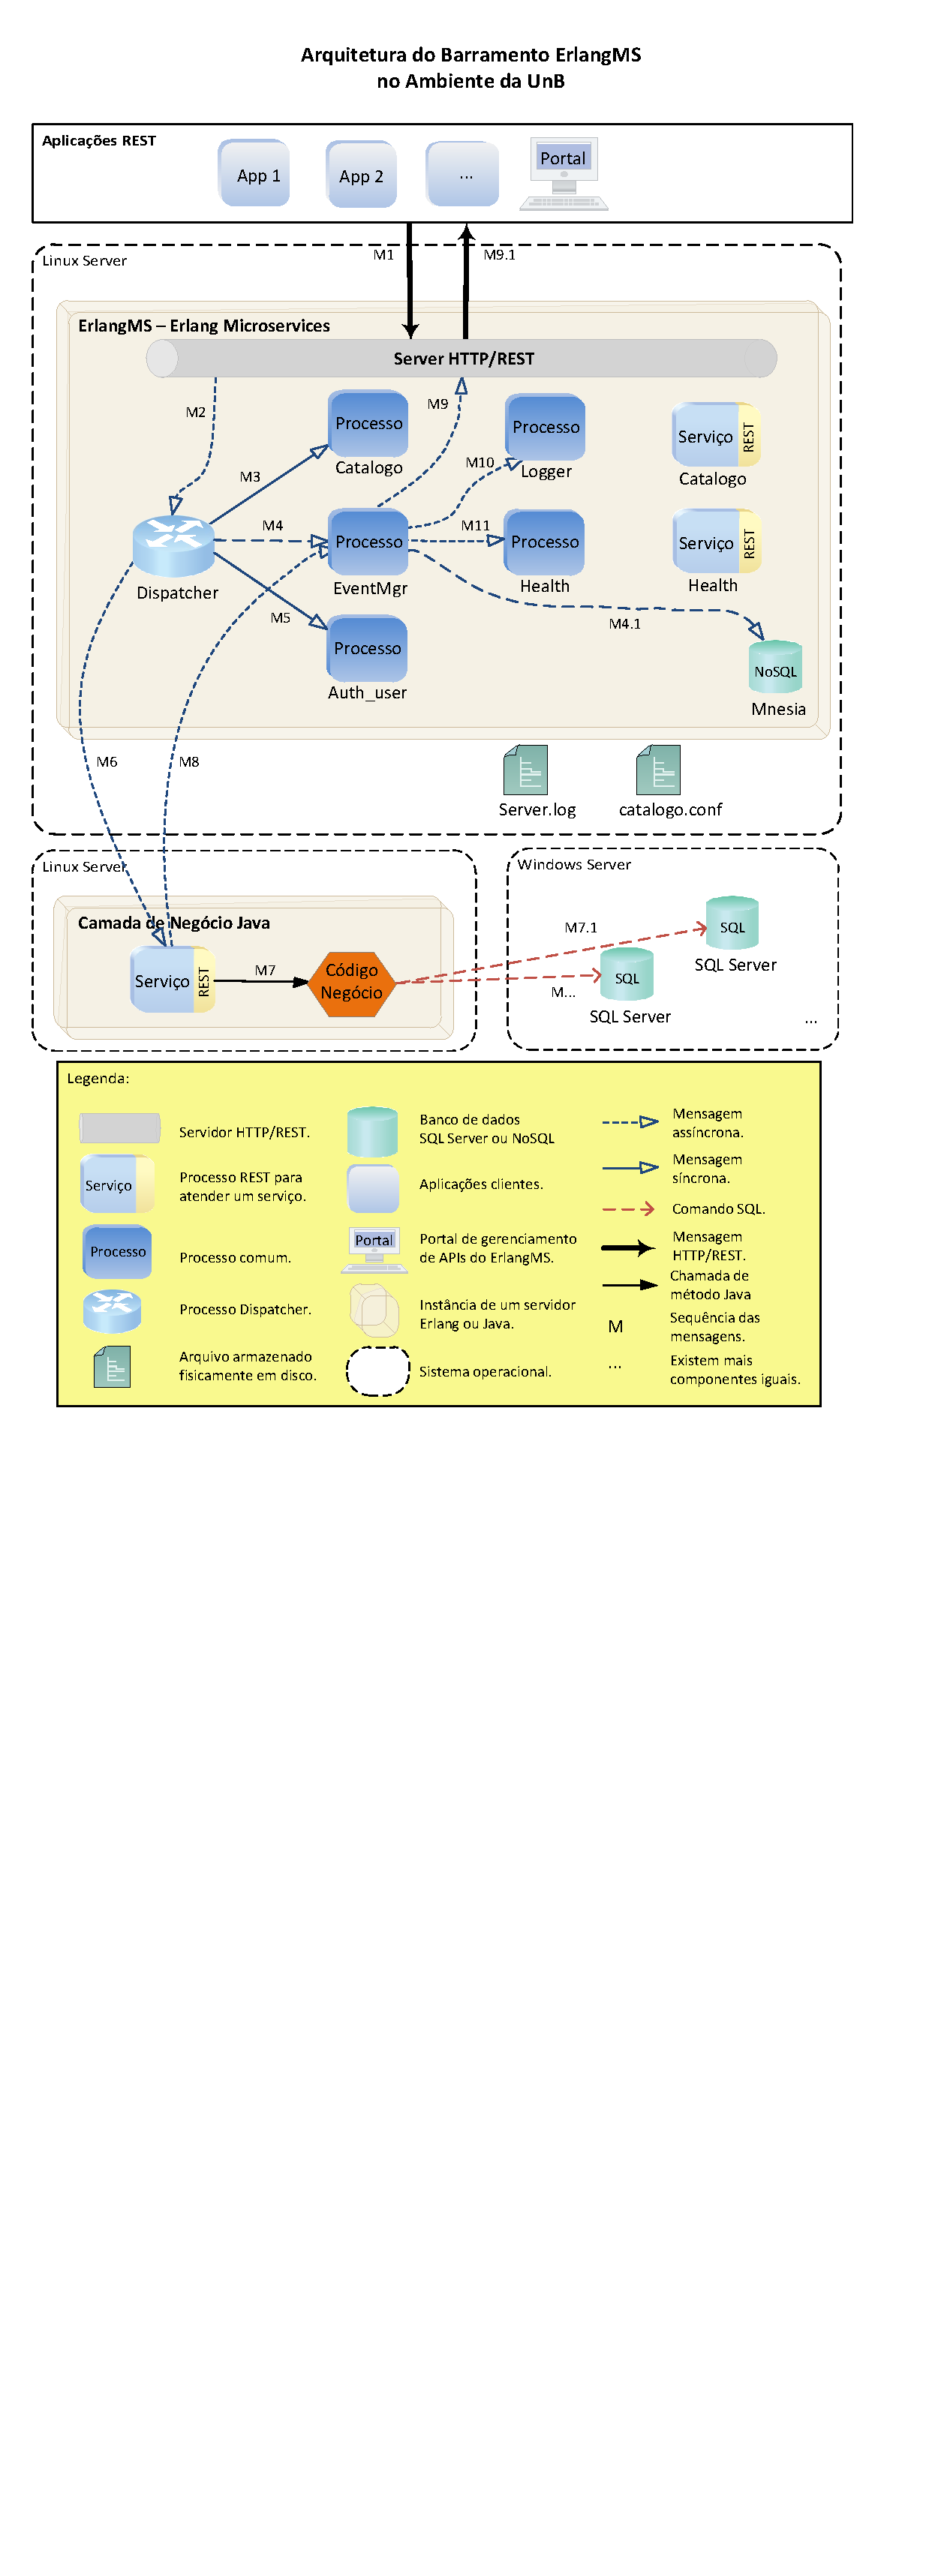
\includegraphics[scale=0.71]{/img/arquitetura/arquitetura_erlangms.pdf}
\caption{Vis\~{a}o geral da arquitetura proposta.}
\label{fig:arquitetura}
\end{figure}
